% ============================================================================
%  Doc C -- SPEAR3 LLRF Upgrade: Interface Chassis and Waveform Buffer
%           Design Requirements
%  Build:  powershell -ExecutionPolicy Bypass -File build.ps1 -Doc C
%  Engine: LuaLaTeX (required -- see the Unicode note in preamble.tex)
% ============================================================================
\documentclass[letterpaper,11pt]{article}
% ============================================================================
%  SPEAR3 RF System documentation -- shared preamble
%  Engine: LuaLaTeX.  Build with build.ps1 (latexmk -lualatex).
% ============================================================================

\usepackage[letterpaper,top=1in,bottom=1in,left=1.05in,right=1.05in]{geometry}

% --- fonts -----------------------------------------------------------------
\usepackage{fontspec}
\setmainfont{TeX Gyre Termes}
\setsansfont{TeX Gyre Heros}
\setmonofont{Consolas}[Scale=0.86]

% --- Unicode safety --------------------------------------------------------
% LuaLaTeX DROPS unmapped glyphs SILENTLY -- an unmapped U+03BC turns "8 uF"
% into "8 F".  Every non-ASCII character used in these documents is mapped
% here.  The build script fails if the log reports "Missing character".
\usepackage{newunicodechar}
\newunicodechar{μ}{\ensuremath{\mu}}      \newunicodechar{µ}{\ensuremath{\mu}}
\newunicodechar{Ω}{\ensuremath{\Omega}}   \newunicodechar{≈}{\ensuremath{\approx}}
\newunicodechar{≥}{\ensuremath{\geq}}     \newunicodechar{≤}{\ensuremath{\leq}}
\newunicodechar{≠}{\ensuremath{\neq}}     \newunicodechar{×}{\ensuremath{\times}}
\newunicodechar{÷}{\ensuremath{\div}}     \newunicodechar{±}{\ensuremath{\pm}}
\newunicodechar{−}{\ensuremath{-}}        \newunicodechar{√}{\ensuremath{\sqrt{}}}
\newunicodechar{α}{\ensuremath{\alpha}}   \newunicodechar{β}{\ensuremath{\beta}}
\newunicodechar{φ}{\ensuremath{\varphi}}  \newunicodechar{ω}{\ensuremath{\omega}}
\newunicodechar{Δ}{\ensuremath{\Delta}}   \newunicodechar{τ}{\ensuremath{\tau}}
\newunicodechar{θ}{\ensuremath{\theta}}   \newunicodechar{λ}{\ensuremath{\lambda}}
\newunicodechar{π}{\ensuremath{\pi}}      \newunicodechar{σ}{\ensuremath{\sigma}}
\newunicodechar{₀}{\ensuremath{_0}}       \newunicodechar{₁}{\ensuremath{_1}}
\newunicodechar{₂}{\ensuremath{_2}}       \newunicodechar{²}{\ensuremath{^2}}
\newunicodechar{³}{\ensuremath{^3}}       \newunicodechar{⁴}{\ensuremath{^4}}
\newunicodechar{⁻}{\ensuremath{^-}}       \newunicodechar{⁺}{\ensuremath{^+}}
\newunicodechar{→}{\ensuremath{\rightarrow}}
\newunicodechar{←}{\ensuremath{\leftarrow}}
\newunicodechar{↔}{\ensuremath{\leftrightarrow}}
\newunicodechar{⇒}{\ensuremath{\Rightarrow}}
\newunicodechar{⊕}{\ensuremath{\oplus}}   \newunicodechar{∥}{\ensuremath{\parallel}}
\newunicodechar{°}{\ensuremath{^\circ}}   \newunicodechar{·}{\ensuremath{\cdot}}
\newunicodechar{≪}{\ensuremath{\ll}}      \newunicodechar{≫}{\ensuremath{\gg}}
\newunicodechar{✓}{\checkmark}            \newunicodechar{⚠}{\textbf{!}}
\newunicodechar{–}{--}                    \newunicodechar{—}{---}

% --- maths and units -------------------------------------------------------
\usepackage{amsmath,amssymb}
\usepackage{siunitx}
\DeclareSIUnit\voltampere{VA}
\DeclareSIUnit\VAR{var}
% range-phrase must not rely on literal spaces (LaTeX strips them from a key
% value, so "{ to }" renders as "10to20") and must force text mode (siunitx
% sets numbers in math, where a bare "--" becomes two minus signs).
\sisetup{per-mode=symbol,range-phrase={\text{--}},range-units=single,
         group-minimum-digits=4,detect-weight=true}

% --- tables ----------------------------------------------------------------
\usepackage{longtable,booktabs,array,tabularx,multirow}
\usepackage{ragged2e}
\setlength{\LTleft}{0pt}\setlength{\LTright}{0pt}
\renewcommand{\arraystretch}{1.18}
% left-aligned, hyphenating paragraph column used by every wide table
\newcolumntype{P}[1]{>{\RaggedRight\arraybackslash}p{#1}}
% Same, but \small: for dense tables.  The size must live in the column type --
% wrapping a longtable in {\small ...} breaks its page-breaking \write.
\newcolumntype{Q}[1]{>{\small\RaggedRight\arraybackslash}p{#1}}

% --- graphics and figures --------------------------------------------------
\usepackage{graphicx}
% Resolved from the document's own folder, which is the working directory.
\graphicspath{{../common/}{../common/photos/}{../common/generated/}}
\usepackage{float}
\usepackage[font=small,labelfont=bf,width=0.92\linewidth]{caption}
\usepackage{comment}
% longtable* (from ltcaption, loaded by caption) is for tables without a caption,
% but longtable still steps the table counter.  Give it a private anchor and take
% the number back, so the numbered tables run 1, 2, 3 and their links are unique.
\makeatletter
\AddToHook{env/longtable*/begin}{\def\theHtable{nocap.\arabic{LT@tables}}}
\AddToHook{env/longtable*/after}{\addtocounter{table}{-1}}
\makeatother

% A figure must not drift out of the section it belongs to.  With 47 floats
% LaTeX will otherwise push them pages away from the text that discusses them.
\usepackage[section]{placeins}

% Default float parameters are tuned for papers with two or three figures.
% This document is figure-dense, so allow more of a page to be float and more
% floats per page; without this, figures queue up and drift several pages.
\renewcommand{\topfraction}{0.88}
\renewcommand{\bottomfraction}{0.70}
\renewcommand{\textfraction}{0.10}
\renewcommand{\floatpagefraction}{0.72}
\setcounter{topnumber}{3}
\setcounter{bottomnumber}{2}
\setcounter{totalnumber}{5}

% Image size policy.  Photographs are capped in BOTH width and height so that
% no figure can ever exceed roughly half a page, whatever its aspect ratio.
\newlength{\photomaxh}\setlength{\photomaxh}{0.34\textheight} % ~1/3 page
\newlength{\widemaxh} \setlength{\widemaxh}{0.46\textheight}  % ~1/2 page

% \photofig{file}{caption}{label}      -- default, about 1/3 page
\newcommand{\photofig}[3]{%
  \begin{figure}[htbp]\centering
    \includegraphics[width=0.62\linewidth,height=\photomaxh,keepaspectratio]{#1}%
    \caption{#2}\label{#3}
  \end{figure}}
% \widefig{file}{caption}{label}       -- for detailed schematics, about 1/2 page
\newcommand{\widefig}[3]{%
  \begin{figure}[htbp]\centering
    \includegraphics[width=0.94\linewidth,height=\widemaxh,keepaspectratio]{#1}%
    \caption{#2}\label{#3}
  \end{figure}}
% \smallfig{file}{caption}{label}      -- for low-resolution sources
\newcommand{\smallfig}[3]{%
  \begin{figure}[htbp]\centering
    \includegraphics[width=0.44\linewidth,height=0.26\textheight,keepaspectratio]{#1}%
    \caption{#2}\label{#3}
  \end{figure}}
% \tallfig{file}{caption}{label}       -- portrait-orientation photographs.
% A tall photo capped at \photomaxh comes out only ~45 mm wide, so these are
% capped by height instead and allowed a narrower column.
\newcommand{\tallfig}[3]{%
  \begin{figure}[tbp]\centering
    \includegraphics[width=0.46\linewidth,height=0.4\textheight,keepaspectratio]{#1}%
    \caption{#2}\label{#3}
  \end{figure}}
% two portrait photographs side by side under one caption:
% \tallpairfig{fileA}{subA}{labA}{fileB}{subB}{labB}{caption}{label}
\newcommand{\tallpairfig}[8]{%
  \begin{figure}[tbp]\centering
    \begin{minipage}[b]{0.46\linewidth}\centering
      \includegraphics[width=\linewidth,height=0.40\textheight,keepaspectratio]{#1}%
      \subcaption{#2}\label{#3}
    \end{minipage}\hfill
    \begin{minipage}[b]{0.46\linewidth}\centering
      \includegraphics[width=\linewidth,height=0.40\textheight,keepaspectratio]{#4}%
      \subcaption{#5}\label{#6}
    \end{minipage}
    \caption{#7}\label{#8}
  \end{figure}}
% two photographs side by side, each about 1/4 page
\newcommand{\pairfig}[6]{%
  \begin{figure}[htbp]\centering
    \begin{minipage}[t]{0.48\linewidth}\centering
      \includegraphics[width=\linewidth,height=0.26\textheight,keepaspectratio]{#1}%
      \subcaption{#2}\label{#3}
    \end{minipage}\hfill
    \begin{minipage}[t]{0.48\linewidth}\centering
      \includegraphics[width=\linewidth,height=0.26\textheight,keepaspectratio]{#4}%
      \subcaption{#5}\label{#6}
    \end{minipage}
  \end{figure}}
\usepackage{subcaption}

% --- diagrams --------------------------------------------------------------
\usepackage{tikz}
\usetikzlibrary{arrows.meta,positioning,fit,backgrounds,calc,shapes.geometric,
                shapes.misc,chains,decorations.pathreplacing,patterns,matrix}
\usepackage{pgfplots}\pgfplotsset{compat=1.18}
\usepackage{rotating}                  % sidewaysfigure, if a portrait page is wanted
\usepackage{pdflscape}                 % landscape: rotates the PAGE in the PDF
\usepackage[export]{adjustbox}         % max width= / max height= on a box

% Shrink a diagram to the text width only if it would otherwise overflow, so
% figures drawn at their natural scale are never enlarged or needlessly shrunk.
\newsavebox{\fitbox}
\newenvironment{fitpicture}
  {\begin{lrbox}{\fitbox}}
  {\end{lrbox}%
   \ifdim\wd\fitbox>\linewidth
     \resizebox{\linewidth}{!}{\usebox{\fitbox}}%
   \else
     \usebox{\fitbox}%
   \fi}

% House diagram style.  Keep every block diagram in these styles so the
% document reads as one drawing set rather than a scrapbook.
\definecolor{cCtrl}{HTML}{1F4E79}   % control / EPICS
\definecolor{cPlc} {HTML}{7F6000}   % PLC / interlock
\definecolor{cPwr} {HTML}{843C0C}   % high power
\definecolor{cRf}  {HTML}{2E6B34}   % RF signal path
\definecolor{cNeut}{HTML}{3B3B3B}
\tikzset{
  blk/.style   ={draw=cNeut,fill=white,rounded corners=1.6pt,align=center,
                 inner sep=4pt,font=\scriptsize,minimum height=8mm},
  ctrl/.style  ={blk,draw=cCtrl,fill=cCtrl!7,text=cCtrl!85!black},
  plc/.style   ={blk,draw=cPlc, fill=cPlc!8, text=cPlc!80!black},
  pwr/.style   ={blk,draw=cPwr, fill=cPwr!7, text=cPwr!85!black},
  rf/.style    ={blk,draw=cRf,  fill=cRf!7,  text=cRf!80!black},
  grp/.style   ={draw=black!35,dashed,rounded corners=3pt,inner sep=7pt},
  lbl/.style   ={font=\scriptsize\itshape,text=black!62},
  sig/.style   ={-{Stealth[length=2.2mm]},draw=cNeut,thick},
  fib/.style   ={sig,densely dashed},
  bus/.style   ={draw=cNeut,line width=1.1pt},
  tag/.style   ={font=\tiny,inner sep=1.4pt,fill=white,text=black!70},
}
% consistent caption for a TikZ figure
\newcommand{\diagcap}[2]{\caption{#1}\label{#2}}

% --- lists, misc -----------------------------------------------------------
\usepackage{enumitem}
\setlist{nosep,leftmargin=1.35em}
\providecommand{\tightlist}{%   emitted by pandoc for compact lists
  \setlength{\itemsep}{0pt}\setlength{\parskip}{0pt}}
\usepackage[table]{xcolor}
\usepackage{soul}
\usepackage{microtype}
\usepackage{fancyhdr}
\usepackage{lastpage}
\usepackage{needspace}

% --- callout box for warnings / key findings -------------------------------
\usepackage[most]{tcolorbox}
\newtcolorbox{keynote}[1][]{colback=black!3,colframe=black!45,boxrule=0.4pt,
  arc=1.5pt,left=5pt,right=5pt,top=4pt,bottom=4pt,fontupper=\small,#1}
\newtcolorbox{warnbox}[1][]{colback=cPwr!5,colframe=cPwr!70,boxrule=0.7pt,
  arc=1.5pt,left=5pt,right=5pt,top=4pt,bottom=4pt,fontupper=\small,#1}

% --- cross references and links --------------------------------------------
\usepackage[hyphens]{url}
\usepackage[hidelinks,pdfusetitle,bookmarksnumbered]{hyperref}
\usepackage[capitalise,nameinlink]{cleveref}
\crefname{section}{\S}{\S\S}
\Crefname{section}{Section}{Sections}
% Spell out "Figure" for \cref too; cleveref's default abbreviates it to "Fig.",
% which reads inconsistently beside \Cref in the same sentence.
\crefname{figure}{Figure}{Figures}
% Lowercase \cref on a section prints "§5.7" / "§§10.2--10.5" -- no space after
% the sign and an en-dash range, matching the hand-written style it replaced.
\crefformat{section}{\S#2#1#3}
\crefrangeformat{section}{\S\S#3#1#4--#5#2#6}
\crefmultiformat{section}{\S#2#1#3}{ and~\S#2#1#3}{, \S#2#1#3}{ and~\S#2#1#3}

% Repository paths are long and unhyphenatable; allow breaks after / and .
% Long file paths and CamelCase document names have no natural break points, so
% url's default break set is not enough: allow a break before any capital and
% after the usual separators.
\newcommand{\fpath}[1]{{\ttfamily\small\Urlmuskip=0mu plus 1mu\relax
  \def\UrlBreaks{\do\/\do\.\do\-\do\_\do\:\do\A\do\B\do\C\do\D\do\E\do\F\do\G
    \do\H\do\I\do\J\do\K\do\L\do\M\do\N\do\O\do\P\do\Q\do\R\do\S\do\T\do\U
    \do\V\do\W\do\X\do\Y\do\Z}%
  \urlstyle{tt}\nolinkurl{#1}}}
\setlength{\emergencystretch}{2em}

% --- headers ---------------------------------------------------------------
\pagestyle{fancy}\fancyhf{}
\renewcommand{\headrulewidth}{0.3pt}
\fancyhead[L]{\footnotesize\nouppercase{\rightmark}}
\fancyhead[R]{\footnotesize\thepage\ / \pageref{LastPage}}
\renewcommand{\sectionmark}[1]{\markright{\thesection\quad #1}}
\fancypagestyle{plain}{\fancyhf{}\renewcommand{\headrulewidth}{0pt}%
  \fancyfoot[C]{\footnotesize\thepage}}

\setcounter{tocdepth}{2}
\setcounter{secnumdepth}{3}


% [Rn] source index: \R{n} links to the row \RDEF{n} in Appendix A.
\DeclareRobustCommand{\R}[1]{\hyperlink{ref:R#1}{[R#1]}}
\DeclareRobustCommand{\RDEF}[1]{%
  \raisebox{0pt}[0pt][0pt]{\hypertarget{ref:R#1}{}}\textbf{[R#1]}}

% Open-item tag: links forward to the register; the register links back here.
\DeclareRobustCommand{\openitem}[1]{\,%
  \raisebox{0pt}[0pt][0pt]{\hypertarget{open:#1}{}}\label{openp:#1}%
  \hyperlink{openitems}{\textcolor{cPlc}{\bfseries\scriptsize[#1]}}}
\newcommand{\openpage}[1]{\hyperlink{open:#1}{p.~\pageref*{openp:#1}}}
\newcommand{\openitemlegend}{\textcolor{cPlc}{\bfseries\scriptsize[O\textit{n}]}}

% Column width for longtables with @{} edges: fraction of \linewidth minus the
% per-column share of the inter-column padding, 2(n-1)/n \tabcolsep.
\newcommand{\cw}[2]{\dimexpr #1\linewidth-#2\tabcolsep\relax}

% Logic symbols used in the equations of the logic section.
\newcommand{\sig}[1]{\mathit{#1}}

\hypersetup{pdftitle={SPEAR3 LLRF Upgrade: Interface Chassis and Waveform Buffer Design Requirements},
  pdfauthor={Faya Wang},pdfsubject={Doc C R0 - Draft for review}}

\title{\vspace{-1.4cm}\bfseries SPEAR3 LLRF Upgrade\\[2mm]
       \Large Interface Chassis and Waveform Buffer\\ Design Requirements}
\author{}
\date{}

\begin{document}
\maketitle
\thispagestyle{plain}

\begin{center}
\begin{minipage}{0.86\linewidth}\small
\begin{tabular}{@{}ll@{}}
\textbf{Document ID}    & Doc C \\
\textbf{Revision}       & R0 \\
\textbf{Status}         & Draft \\
\textbf{Author}         & Faya Wang \\
\textbf{Reviewer}       & Jim Sebek, D.~Zhang \\
\textbf{Classification} & Tier 2 --- Subsystem design requirements \\
\textbf{Affiliation}    & SSRL, SLAC National Accelerator Laboratory \\
\textbf{Date}           & 10 November 2026 \\
\end{tabular}
\end{minipage}
\end{center}

\vspace{4mm}
\begin{keynote}
This document sets the design requirements of the Interface Chassis and the Waveform
Buffer, the two boards of one chassis in the SPEAR3 LLRF Upgrade: every input and
output with its medium, level and sense; the logic that forms the permits, written
from the required behavior of the system; latching, reset and first-fault recording;
timing and fail-safe states; the Waveform Buffer channels, buffers, comparators and
collector-power trip; status reporting to the RF MPS and EPICS; and verification. It
covers the transition period, when the chassis replaces the Fast Interlock Chassis and
the RF Local Display Panel while the legacy station is still in service, and the end
state. Statements that still need confirmation are tagged \openitemlegend{} and
collected in the \hyperref[sec:open-items]{Open Items} register; values marked
\emph{proposed} are for review.
\end{keynote}

\clearpage
\tableofcontents
\clearpage

% !TeX root = C_interface_chassis_requirements.tex
% Body of Doc C.  Edit THIS file for content changes; the main file holds only
% the preamble, title block and table of contents.

% ===========================================================================
\section*{Revision History}
\markboth{Revision History}{Revision History}
\addcontentsline{toc}{section}{Revision History}\label{revision-history}

\begin{longtable*}[c]{@{}Q{\cw{0.10}{1.5}}Q{\cw{0.14}{1.5}}Q{\cw{0.18}{1.5}}Q{\cw{0.58}{1.5}}@{}}
\toprule
Revision & Date & Scope of Change & Summary \\
\midrule
\endhead
\bottomrule
\endlastfoot
\textbf{R0} & 2026-11-13 & Draft for review & Initial issue: requirements of both
boards for the transition period and the end state; decisions D1 to D13. \\
\end{longtable*}

% R0 drafting notes, not rendered (frozen):
% Initial issue: interfaces, signal levels, permit logic written from the required
% behavior of the system, latching, reset and first fault, timing and fail-safe
% states, Waveform Buffer channels, buffers, comparators and collector-power trip,
% status reporting and verification, for the transition period and the end state.
% Every signal checked against the drawings of the panel, the Fast Interlock Chassis
% and the AIM: the X530 lines that the panel only displays are not taken over, nor
% are the key switches, which operators do not use, or the beam-abort output, which
% nothing at SPEAR3 receives. VXI Slot 5 stays until I8; the chassis takes the SPEAR
% MPS and orbit permits in parallel from I2 and drives the AIM's External MPS channel
% in place of Slot 5's J3 (D7). The Waveform Buffer's HVPS channels 3 and 4 take the
% transformer current and the SCR firing signal of the B118 oscilloscope.
% 12 November, after review: the LLRF9 enable is held on from I2, in place of the
% 2021 LLRF Window Interlock Status chassis, and follows the logic from I3 (D8); the
% AIM's beam-abort command is not connected (D4); neither the HVPS controller nor the
% chassis sends a heartbeat, and the reset and status lines serve the ControlLogix
% from I4 (D9); the arc lines to the AIM are only terminated, and the chassis IOC
% reports the arcs (ST-7); the two boards are the interlock board and the Waveform
% Buffer board; Waveform Buffer channel 1 takes waveguide load 1 forward, whose LLRF9
% input goes to the klystron drive (Doc 0), and the channel assignment is settled, so
% O8 is closed and O9 becomes O8.  Later 12 November: text made more concise; the RF
% MPS reset and status lines (M3, M4) and the Waveform Buffer external trigger dropped
% (D10, D11); the buffers freeze on any input latch.
% 13 November: the RF MPS summary permit acts from I2 and the heartbeat only alarms
% (D2); the LLRF9 outputs act from I6 (D12); M1 and M2 became P5 and P6; O9 added.
% Later 13 November: the chassis IOC resets the LLRF9 after each chassis reset (ST-8)
% and freezes the Waveform Buffer on a legacy RF fault (ST-9); processor commands to
% the boards in CH-3 and Fig 1; D2 rationale.
% Later 13 November: section Station Shut-Off and Reset (tab:latches, tab:shutoff,
% RS-1 to RS-4) replaces the recovery subsection, from rf_states.st, the station
% records and the HVPS controller program (R27): STATUS follows the contactor, not
% the trigger enable; the controller's SCR ON latch sets only within 0.5 s of the
% trigger enable; the reset sequence ends the HVPS reset after 2 s. D2 rationale
% limited to the documented paths; O4 adds when the AIM drops HVPS_ON.
% Then: a crowbar makes the HVPS controller open its contactor (R27, rungs 0002 and
% 0013), so STATUS stays dark until the contactor closes again (tab:shutoff); the 2021
% LLRF Window Interlock Status chassis row removed from tab:takeover.
% Then: the 2021 chassis no longer mentioned (scope, LLRF9 section, D8); O1 regains
% its needed-before and page entries.
% Then: section 2 opens with the legacy and I2 connections (fig:stations).
% Then: the LLRF9 spare (HVPS-interlock) outputs L3 and L4 dropped (D13): slow-ADC
% events also trip the unit and reach the chassis on L2. Fig 3 declared at the start
% of section 5. Review fixes: status goes to EPICS, not the RF MPS (tab:takeover);
% the AIM drives 21 J15 lines; display-only O:030/17 (J3-22); STATUS dark after a
% crowbar (sec:io-hvps); arc receivers J17 to J28.
% Then: Fig 1 shows the twelve arc-detector fibers on the Fast Interlock Chassis (a)
% and on the ARC4 from I1 (b); caption and section 2 say so.

% ===========================================================================
\section*{Open Items --- Still To Be Confirmed}
\markboth{Open Items}{Open Items}
\addcontentsline{toc}{section}{Open Items --- Still To Be Confirmed}\label{sec:open-items}
\raisebox{0pt}[0pt][0pt]{\hypertarget{openitems}{}}

Each item is tagged \openitemlegend{} where a requirement depends on it; the page
column links to that point. Where an item is the same as one of Doc~0 or Doc~M, that
item is named.

\begin{longtable*}[c]{@{}Q{\cw{0.06}{1.6}}Q{\cw{0.15}{1.6}}Q{\cw{0.47}{1.6}}Q{\cw{0.22}{1.6}}Q{\cw{0.10}{1.6}}@{}}
\toprule
ID & Item & What is needed & Needed before & Page \\
\midrule
\endhead
\bottomrule
\endlastfoot
O1 & Logic equations & The equations of \cref{sec:logic} are written from our
understanding of the system's required behavior, not recovered from the panel's
GAL22V10. & Logic design freeze (I2) & \openpage{O1} \\
O2 & LLRF9 input option & The factory-set logic level of the interlock inputs of the
installed LLRF9 units: \qty{3.3}{\volt}, \qty{5}{\volt} or \qty{24}{\volt} (Doc~0
O1). & Board design & \openpage{O2} \\
O3 & ARC4 interface & The lines of the two system modules and the test module: their
number, levels, the form of the fired-detector identity (parallel bits or an encoded
word), the latch reset and the test lines (Doc~0 O4). & Board layout &
\openpage{O3} \\
O4 & Legacy AIM and Fast IC signals & Confirm on the hardware the J15 levels and
sense that the drawings give (\cref{tab:aim}) and the levels on the 37-pin cable
(\cref{sec:io-j4}), and measure the length of the reset and
timeout-bypass pulses, and record when the AIM drops HVPS\_ON: on a fault, on its forced beam
abort, at a turn-off; the RF level at the detector input J32 and the legacy
detector's transfer curve, on the bench or from archived readings (Doc~M O3). Note: SOLENOID and FILAMENT signals are swapped on Fast Interlock Chassis side (right side of wd3403302900.pdf drawing) & Production
design &
\openpage{O4} \\
O5 & X530 pins & The pin and terminal numbers of the J2 and J3 lines, on which the
drawings disagree, checked by continuity (Doc~M O2). & Cable fabrication &
\openpage{O5} \\
O6 & Heartbeat & The period and duty cycle of the PLC-5 heartbeat at the panel output
and at the AIM input, which set the watchdog timeout (Doc~M O4). & Watchdog design &
\openpage{O6} \\
O7 & SPEAR MPS and orbit permits & Their wiring into VXI Slot~5 and the current
their sources can supply to a second input (Doc~M O6). & Input design (I2) &
\openpage{O7} \\
O8 & HVPS transformer current and SCR firing signal & The pick-off points, amplitudes
and cable route from B118 of the two signals on channels 3 and 4 of the B118
oscilloscope. & Waveform Buffer HVPS inputs (I2) &
\openpage{O8} \\
O9 & RF MPS outputs on a processor fault & Whether the RF MPS outputs, the summary
permit among them, turn off when its processor faults or stops: the PLC-5 I/O chassis
setting and, from I4, the fault setting of the ControlLogix output modules. With the
heartbeat alarm-only, the summary permit is the only trip path from a stopped RF MPS
(D2). & I2 & \openpage{O9} \\
\end{longtable*}

% ===========================================================================
\section{Purpose, Scope and Basis}\label{sec:purpose}

\paragraph{Purpose.} The Interface Chassis is the hardware interlock hub of the
upgraded SPEAR3 RF station: it sums the permits of the subsystems and the external
safety systems, drives the permits to the LLRF9 and the HVPS controller, latches every
fault and records the first one \R{1}, \R{4}. The Waveform Buffer, on the second board of the same chassis,
digitizes the RF and HVPS signals that the LLRF9 does not see, keeps them in circular
buffers that freeze on a fault, and trips through the Interface Chassis on its own
comparators and on the klystron collector power \R{1}, \R{5}. This document sets the
design requirements of both: their functions, every input and output with its medium,
level and sense, the permit logic, timing, fail-safe states, status reporting and
verification. It is the reference for the production review of the chassis and for its bench and installation tests.

\paragraph{Scope.} Both boards, the chassis, its connectors and its EPICS interface.
The chassis is installed at integration I2, in place of the Fast Interlock
Chassis 340-308 and the RF Local Display Panel 340-310, while the AIM, the RFP, VXI
Slot~5, the PLC-5 and the legacy HVPS controllers are still in service; it keeps the same role
through the end state after the VXI crate is retired at I8 \R{3}. Out of scope: the
ARC4, the LLRF9, the HVPS controller, the RF MPS program and the PPS Interface Box.
The chassis carries no personnel-protection function.

\paragraph{Basis.} The upgrade design, Doc~0 \R{1}; the legacy station, Doc~L \R{2};
the integration plan, Doc~M \R{3}; J.~Sebek's specification of the Interface Chassis
and design notes on the Waveform Buffer, the power detectors, the analog components,
the controller interfaces, the MPS requirements and the HVPS fibers
\R{4}--\R{12}; the drawings of the panel, the Fast Interlock Chassis, the AIM and the
RF MPS wiring \R{13}--\R{18}, \R{21}; the decoded RF MPS PLC-5 program \R{19}; the
LLRF9 manual \R{20}.

\paragraph{Conventions.}
\begin{itemize}
\item A requirement carries an ID and uses ``shall''. IC marks the interlock board,
LG its logic, WB the Waveform Buffer board, ST status reporting and EPICS, CH
the chassis. Values marked \emph{proposed} are design proposals for review.
\item Every permit is active-high: \qty{24}{\volt} present, a lit fiber or a high
LLRF9 output gives the permit, so a broken cable, a dark fiber or a lost supply
removes it \R{1}, \R{8}. The light conventions of the legacy fibers are kept.
\item A permit that is removed latches as a fault until a reset; a reset never clears
a fault whose cause is still present.
\item Integration numbers I2 to I8 and test numbers are those of Doc~M \R{3}.
\end{itemize}

\paragraph{Terms.}
\begin{description}
\item[Permit input] An input that must be present for some output to give its
permit.
\item[Command input] An input that requests an action, such as the HVPS-on request; it
does not latch.
\item[Act mask] A hardware selection, one per input, that decides whether the input
acts on the outputs. An input whose mask is off is still read, latched and reported
(monitor-only).
\item[Transition interface] An interface of the Fast Interlock Chassis or the local panel
that the chassis must present while the legacy station is in service.
\end{description}

% Declared here, not in section 2, so that it is not held back behind section 2's long tables.
\begin{figure}[H]
\centering
\begin{fitpicture}
% !TeX root = ../C_interface_chassis_requirements.tex
% Legacy station (a) and the station from I2 (b): the cables and fibers that the
% Interface Chassis takes over. Same columns in both panels; dashed lines are fibers.
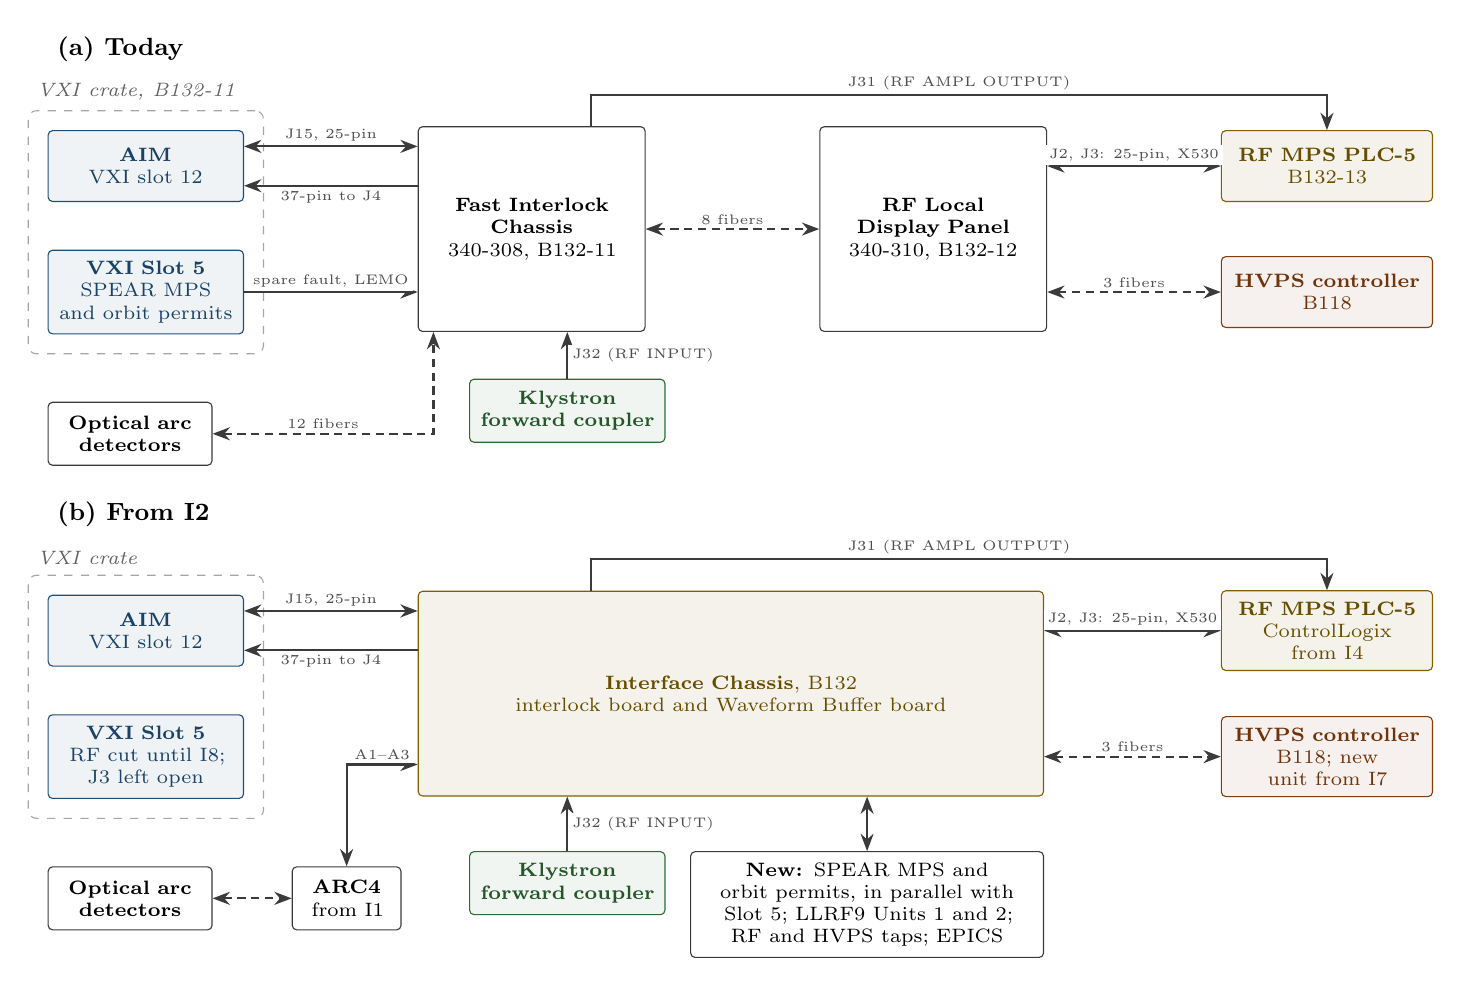
\begin{tikzpicture}[font=\scriptsize, x=1mm, y=1mm,
  every node/.append style={execute at begin node=\hyphenpenalty 10000\relax},
  vxi/.style={ctrl,text width=22mm,minimum height=9mm,anchor=west},
  endbox/.style={text width=24mm,minimum height=9mm,anchor=west},
  two/.style={sig,{Stealth[length=2.2mm]}-{Stealth[length=2.2mm]}},
  twof/.style={fib,{Stealth[length=2.2mm]}-{Stealth[length=2.2mm]}}]

% ===== (a) today =============================================================
\node[anchor=south west,font=\small\bfseries] at (0,4) {(a) Today};
\node[vxi] (aaim) at (0,-8)  {\textbf{AIM}\\ VXI slot~12};
\node[vxi] (as5)  at (0,-24) {\textbf{VXI Slot~5}\\ SPEAR MPS and orbit permits};
\begin{scope}[on background layer]
  \node[grp,fit=(aaim)(as5)] (avxi) {};
\end{scope}
\node[lbl,anchor=south west] at (avxi.north west) {VXI crate, B132-11};
\node[blk,text width=26mm,minimum height=26mm,anchor=west] (afic) at (47,-16)
  {\textbf{Fast Interlock Chassis}\\ 340-308, B132-11};
\node[blk,text width=26mm,minimum height=26mm,anchor=west] (apan) at (98,-16)
  {\textbf{RF Local Display Panel}\\ 340-310, B132-12};
\node[plc,endbox] (aplc) at (149,-8)  {\textbf{RF MPS PLC-5}\\ B132-13};
\node[pwr,endbox] (ahv)  at (149,-24) {\textbf{HVPS controller}\\ B118};
\node[rf,text width=22mm,anchor=north] (akf) at (66,-35)
  {\textbf{Klystron}\\ \textbf{forward coupler}};
\node[blk,text width=18mm,anchor=west] (adet) at (0,-42)
  {\textbf{Optical arc}\\ \textbf{detectors}};

\draw[two] (aaim.east |- 0,-5.5) -- (afic.west |- 0,-5.5) node[tag,midway,above]{J15, 25-pin};
\draw[sig] (afic.west |- 0,-10.5) -- (aaim.east |- 0,-10.5) node[tag,midway,below]{37-pin to J4};
\draw[sig] (as5.east) -- (as5.east -| afic.west) node[tag,midway,above]{spare fault, LEMO};
\draw[twof] (afic.east) -- (apan.west) node[tag,midway,above]{8 fibers};
\draw[two] (apan.east |- aplc.west) -- (aplc.west) node[tag,midway,above]{J2, J3: 25-pin, X530};
\draw[twof] (apan.east |- ahv.west) -- (ahv.west) node[tag,midway,above]{3 fibers};
\draw[sig] (akf.north) -- (akf.north |- afic.south) node[tag,midway,right]{J32 (RF INPUT)};
\draw[twof] (adet.east) -| ([xshift=2mm]afic.south west)
  node[tag,pos=0.25,above]{12 fibers};
% the J31 cable runs over the panel to the PLC-5's analog input
\draw[sig] ([xshift=22mm]afic.north west) -- ++(0,4) -| (aplc.north)
  node[tag,pos=0.25,above]{J31 (RF AMPL OUTPUT)};

% ===== (b) from I2 ===========================================================
\node[anchor=south west,font=\small\bfseries] at (0,-55) {(b) From I2};
\node[vxi] (baim) at (0,-67) {\textbf{AIM}\\ VXI slot~12};
\node[vxi] (bs5)  at (0,-83) {\textbf{VXI Slot~5}\\ RF cut until I8;\\ J3 left open};
\begin{scope}[on background layer]
  \node[grp,fit=(baim)(bs5)] (bvxi) {};
\end{scope}
\node[lbl,anchor=south west] at (bvxi.north west) {VXI crate};
\node[plc,text width=76.6mm,minimum height=26mm,anchor=west] (bic) at (47,-75)
  {\textbf{Interface Chassis}, B132\\ interlock board and Waveform Buffer board};
\node[plc,endbox] (bplc) at (149,-67) {\textbf{RF MPS PLC-5}\\ ControlLogix from I4};
\node[pwr,endbox] (bhv)  at (149,-83) {\textbf{HVPS controller}\\ B118; new unit from I7};
\node[rf,text width=22mm,anchor=north] (bkf) at (66,-95)
  {\textbf{Klystron}\\ \textbf{forward coupler}};
\node[blk,text width=42mm,anchor=north east] (bnew) at (bic.east |- 0,-95)
  {\textbf{New:} SPEAR MPS and orbit permits, in parallel with Slot~5;
   LLRF9 Units~1 and 2; RF and HVPS taps; EPICS};
\node[blk,text width=18mm,anchor=west] (bdet) at (0,-101)
  {\textbf{Optical arc}\\ \textbf{detectors}};
\node[blk,text width=11mm,anchor=west] (barc) at (31,-101) {\textbf{ARC4}\\ from I1};

\draw[two] (baim.east |- 0,-64.5) -- (bic.west |- 0,-64.5) node[tag,midway,above]{J15, 25-pin};
\draw[sig] (bic.west |- 0,-69.5) -- (baim.east |- 0,-69.5) node[tag,midway,below]{37-pin to J4};
\draw[two] (bic.east |- bplc.west) -- (bplc.west) node[tag,midway,above]{J2, J3: 25-pin, X530};
\draw[twof] (bic.east |- bhv.west) -- (bhv.west) node[tag,midway,above]{3 fibers};
\draw[sig] (bkf.north) -- (bkf.north |- bic.south) node[tag,midway,right]{J32 (RF INPUT)};
\draw[two] (bnew.north) -- (bnew.north |- bic.south);
\draw[twof] (bdet.east) -- (barc.west);
\draw[two] (barc.north) |- (bic.west |- 0,-84) node[tag,pos=0.75,above]{A1--A3};
\draw[sig] ([xshift=22mm]bic.north west) -- ++(0,4) -| (bplc.north)
  node[tag,pos=0.25,above]{J31 (RF AMPL OUTPUT)};
\end{tikzpicture}

\end{fitpicture}
\caption[Connections of the legacy station and of the station from I2.]{Connections of
the legacy station (a) and of the station from I2 (b); dashed lines are fibers. The
Interface Chassis keeps every external cable and fiber of the two legacy units, the RF
cables J32 (RF INPUT) and J31 (RF AMPL OUTPUT) of the forward-power detector among
them (\cref{sec:io-analog}), except the twelve arc-detector fibers, which move to the
ARC4 at I1; ten of them are on test-light transmitters and two on receivers \R{2}. The
eight fibers between the units become internal, and the LEMO cable from Slot~5's J3
is left open (D7). \Cref{fig:context} gives every interface of the
chassis.}\label{fig:stations}
\end{figure}

% ===========================================================================
\section{Role in the Station}\label{sec:role}

Today the AIM in the VXI crate reaches the Fast Interlock Chassis through two cables,
J15 (25-pin) and the 37-pin cable to the AIM's J4, and VXI Slot~5 sends it the
External MPS signal on a LEMO cable. Its detector takes the klystron forward power on
J32 and sends the level to the PLC-5 on J31, and twelve arc-detector fibers end on its
rear. Eight fibers link the Fast Interlock Chassis to
the RF Local Display Panel; the panel reaches the PLC-5 through its two 25-pin
connectors J2 and J3 and cross-connect X530, and the HVPS controller in B118 through
three fibers \R{10}, \R{12}--\R{18}. The arc fibers move to the ARC4 at I1. From I2 the
Interface Chassis takes the place of both legacy units and keeps the AIM cables, the
two RF cables, J2 and J3 and the three HVPS fibers; the
eight fibers between the two units become internal (\cref{fig:stations}).

\Cref{tab:takeover} lists the functions that the chassis takes over from the legacy
units and those that are new; \cref{tab:dropped} lists the legacy signals that it does
not take over.

\begin{longtable}[c]{@{}Q{\cw{0.22}{1.333}}Q{\cw{0.48}{1.333}}Q{\cw{0.30}{1.333}}@{}}
\caption{Functions of the chassis.}\label{tab:takeover}\\
\toprule
From & Function & In the chassis \\
\midrule
\endfirsthead
\toprule
From & Function & In the chassis \\
\midrule
\endhead
\bottomrule
\endlastfoot
Fast Interlock Chassis & The six AIM commands on J15 turned into fibers to the
panel; the AB summary and heartbeat returned to the AIM \R{12} & AIM interface,
without the beam abort, \cref{sec:io-aim} \\
Fast Interlock Chassis & Klystron forward-power detector: RF input J32 and output J31
(``RF AMPL.'') on the rear, cabled to the PLC-5 for its collector-power calculation
\R{12}, \R{14}, \R{18} & Detector, \cref{sec:io-analog} \\
Fast Interlock Chassis & The 37-pin cable to the AIM's J4: the External MPS line and
the twelve arc lines \R{14}, \R{15} & AIM J4 interface, with the arc lines only
terminated, \cref{sec:io-j4} \\
RF Local Display Panel & The logic that forms SCR ENABLE, KLYSTRON CROWBAR and the beam
abort; two latches for the beam abort and the crowbar \R{13} & Permit logic,
\cref{sec:logic} \\
RF Local Display Panel & End of the three HVPS fibers \R{10}, \R{11} & HVPS fibers,
\cref{sec:io-hvps} \\
RF Local Display Panel & The X530 lines that its logic and fibers use; buffering of
the HVPS voltage and current for the PLC-5 \R{13}, \R{16} & PLC-5 interface,
\cref{sec:io-plc} \\
VXI Slot~5 & The SPEAR MPS and orbit permits; the RF cut through RF\_FAULT; the External
MPS signal to the AIM through its J3 \R{2} & Permits taken in parallel from I2 and
External MPS driven by the chassis; Slot~5 keeps the RF cut until I8 (D7,
\cref{sec:io-ext}) \\
AIM, at I8 & The commands to the panel, which the coordinator then sends through the
chassis IOC & Command path, \cref{sec:status} \\
New & Sum of the permits of the RF MPS, the SPEAR MPS, the orbit interlock, the ARC4,
the Waveform Buffer and spare inputs; LLRF9 enable logic and status; first fault; status to
EPICS \R{1}, \R{4} & \Cref{sec:io,sec:logic,sec:status} \\
New & RF and HVPS waveforms, comparators and the collector-power trip \R{5} &
Waveform Buffer, \cref{sec:wfb} \\
\end{longtable}

\begin{longtable}[c]{@{}Q{\cw{0.20}{1.5}}Q{\cw{0.25}{1.5}}Q{\cw{0.21}{1.5}}Q{\cw{0.34}{1.5}}@{}}
\caption{Legacy signals not taken over.}\label{tab:dropped}\\
\toprule
Signal & Legacy connection & Legacy use & Disposition \\
\midrule
\endfirsthead
\toprule
Signal & Legacy connection & Legacy use & Disposition \\
\midrule
\endhead
\bottomrule
\endlastfoot
Arc-detector fibers & Fast Interlock Chassis receivers J17 to J28 \R{2}; analog
signals on the 37-pin cable from its J2 to the AIM's J4 & The AIM's arc comparators
and latches &
The fibers move to the ARC4 at I1 (A1, A2), and the chassis IOC reports the arcs
(ST-7); the arc lines to the AIM's J4 are terminated at their no-arc level (IC-27c)
\R{14}, \R{15} \\
Spare fault & Front LEMO of the Fast Interlock Chassis, cabled to J3 of the VXI Slot~5
MPS Shutoff module & The AIM's External MPS channel, on pin~34 of the 37-pin cable &
Replaced: the chassis drives that line from the permits S1 and S2 (IC-27b); the J3
cable is labeled and left open \R{15}, \R{23} \\
Test light and trip tests & Fiber transmitters J33 to J44; twelve trip-test lines on
J15 & Tests of the legacy arc detectors & Not needed; the ARC4 has its own test (A3)
\\
AIM supplies & J15 pins~4 to 6; pins~35 to 37 of the 37-pin cable & Power for the
Fast Interlock Chassis, through J15 only: it leaves pins~35 to 37 unconnected & Not
connected; the chassis has its own supplies (IC-26, IC-27c) \\
Detector monitor & Front BNC J16 of the Fast Interlock Chassis & Front monitor, not
cabled & No monitor output (IC-35) \\
Display-only lines & X530 J2-06, -09, -10, -11, -19 and -24; the 13 area summaries
on J3 other than waveguide pressure and collector; the J3 spares & The panel's LEDs:
main focus on, filament, timeout, HV and RF detected, bucking coil on, area
summaries & Not connected; the PLC-5 reports these states to EPICS
(\cref{tab:x530}) \\
Local/remote key switch & Panel; X530 J2-12 to PLC-5 input I:030/1 (P12) & Copied to
EPICS only (\fpath{SRF1:STN:KEY:STAT}) & Dropped (D6): P12 is not connected, so the
PLC-5 reads remote \\
Online/offline key switch & Panel logic; X530 J2-25 to PLC-5 input I:031/7 (P11) &
SCR ENABLE; with the station-online request, the PLC-5's online bit & Replaced (D6):
P11 is held on, and the station-online command from EPICS acts in the logic as
$c_{ON}$ (IC-36) \\
VXI beam abort & J15 pin~15 (BEAM\_ABORT), a fiber to the panel & One input of the
panel's beam abort & Not connected (D4, IC-20): with no beam-abort output it has no
use \R{13}, \R{14} \\
Beam-abort output & Panel logic, latched until reset; rear BNC J6 & The PEP-II
beam-abort system \R{24} & Dropped (D4): J6 is not cabled at SPEAR3, and the SPEAR MPS
takes no status from the RF in hardware \R{4} \\
\end{longtable}

The interfaces come into use in steps (\cref{tab:phases}). Every end-state input is
built in from the start, read and latched, and acts only when its integration has
gone in and its act mask is set \R{3}.

\begin{longtable}[c]{@{}Q{\cw{0.30}{1.714}}Q{\cw{0.12}{1.714}}Q{\cw{0.11}{1.714}}Q{\cw{0.11}{1.714}}Q{\cw{0.12}{1.714}}Q{\cw{0.12}{1.714}}Q{\cw{0.12}{1.714}}@{}}
\caption{Use of the interfaces by integration. A: acts on the outputs; M: read,
latched and reported only; On: held on, without logic; ---: not
connected.}\label{tab:phases}\\
\toprule
Interface & I2 & I3 & I4, I5 & I6 & I7 & I8 on \\
\midrule
\endfirsthead
\toprule
Interface & I2 & I3 & I4, I5 & I6 & I7 & I8 on \\
\midrule
\endhead
\bottomrule
\endlastfoot
HVPS fibers & A & A & A & A & A, legacy or new controller & A \\
AIM, J15 & A & A & A & A & A & --- \\
AIM, 37-pin cable to J4 & A & A & A & A & A & --- \\
PLC-5 lines at X530; \mbox{ControlLogix} from I4 & A & A & A & A & A & A \\
HVPS voltage and current buffers & A & A & A & A & A & A \\
Klystron forward-power detector output (PLC-5; \mbox{ControlLogix} from I4) & A & A & A & A
& A & A \\
ARC4 permit & M, then A & A & A & A & A & A \\
Waveform Buffer comparators & M, then A & A & A & A & A & A \\
LLRF9 status (L2) & M & M & M & A & A & A \\
LLRF9 enable & On & A & A & A & A & A \\
SPEAR MPS and orbit permits & M, then A & A & A & A & A & A \\
RF MPS summary permit (P5) & A & A & A & A & A & A \\
RF MPS heartbeat (P6) & M & M & M & M & M & M \\
Expansion ports & --- & --- & --- & as needed & as needed & as needed \\
\end{longtable}

% ===========================================================================
\section{Chassis Architecture}\label{sec:arch}

The Interface Chassis and the Waveform Buffer are one chassis with two boards, the
interlock board and the Waveform Buffer board; the prototype is built and
the Waveform Buffer board was completed in April 2026 \R{1}. \Cref{fig:context} shows
the chassis with every external interface, by partner.

\begin{figure}[p]
\centering
\begin{fitpicture}
% !TeX root = ../C_interface_chassis_requirements.tex
% The Interface Chassis and every external interface. Left: legacy units and the
% RF MPS; right: HVPS, LLRF9, ARC4 and RF sources. Signal IDs are those of
% tab:signals; dashed lines are fibers. All boxes of a side share one anchor x so
% the arrows stay horizontal.
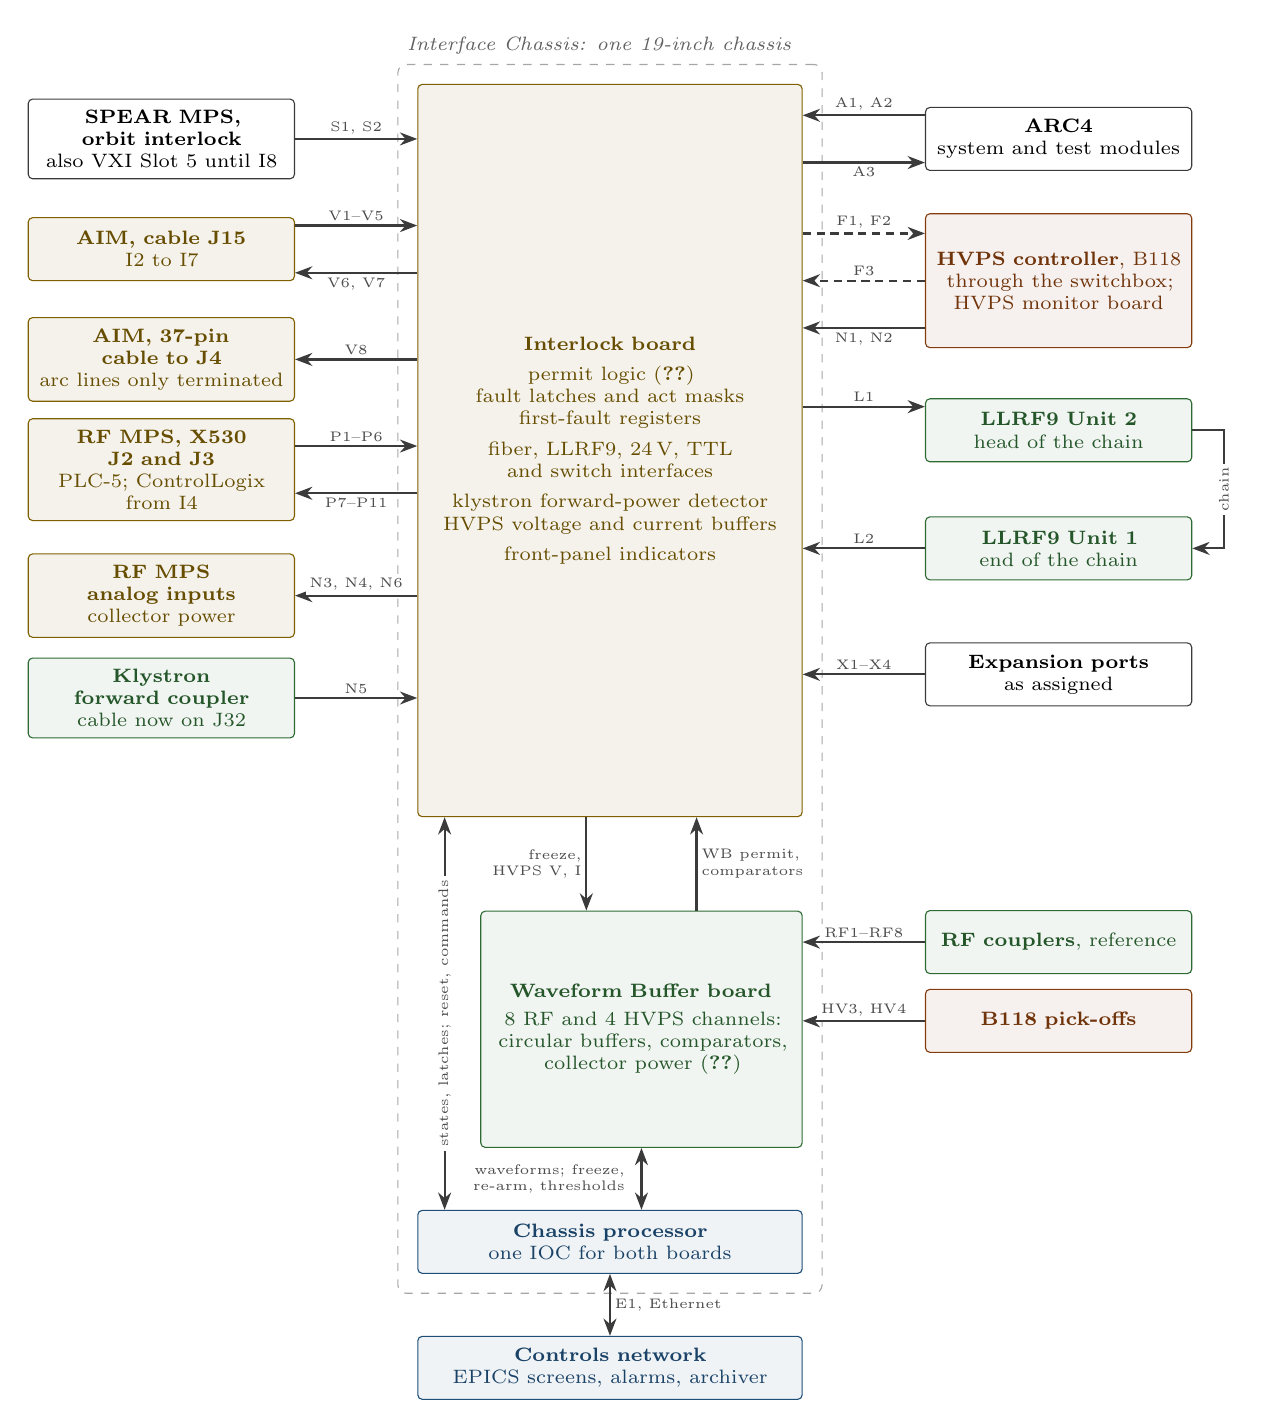
\begin{tikzpicture}[font=\scriptsize, x=1mm, y=1mm,
  every node/.append style={execute at begin node=\hyphenpenalty 10000\relax},
  pl/.style={text width=31mm,anchor=east},
  pr/.style={text width=31mm,anchor=west},
  one/.style={text width=31mm,anchor=west,minimum height=8mm}]

% ----- the chassis -------------------------------------------------------------
\node[plc,text width=46mm,minimum height=93mm,anchor=north] (ib) at (80,-9)
  {\textbf{Interlock board}\\[3pt]
   permit logic (\cref{sec:logic})\\
   fault latches and act masks\\
   first-fault registers\\[3pt]
   fiber, LLRF9, 24\,V, TTL\\ and switch interfaces\\[3pt]
   klystron forward-power detector\\
   HVPS voltage and current buffers\\[3pt]
   front-panel indicators};
\node[rf,text width=38mm,minimum height=30mm,anchor=north] (wb) at (84,-114)
  {\textbf{Waveform Buffer board}\\[2pt]
   8 RF and 4 HVPS channels:\\ circular buffers, comparators,\\
   collector power (\cref{sec:wfb})};
\node[ctrl,text width=46mm,anchor=north] (cpu) at (80,-152)
  {\textbf{Chassis processor}\\ one IOC for both boards};
\node[ctrl,text width=46mm,anchor=north] (net) at (80,-168)
  {\textbf{Controls network}\\ EPICS screens, alarms, archiver};
\begin{scope}[on background layer]
  \node[grp,fit=(ib)(wb)(cpu)] (ch) {};
\end{scope}
\node[lbl,anchor=south west] at (ch.north west) {Interface Chassis: one 19-inch chassis};

% ----- partners on the left ------------------------------------------------------
\node[blk,pl] (smps) at (40,-16) {\textbf{SPEAR MPS, orbit interlock}\\ also VXI Slot~5 until I8};
\node[plc,pl] (j15)  at (40,-30) {\textbf{AIM, cable J15}\\ I2 to I7};
\node[plc,pl] (j4)   at (40,-44) {\textbf{AIM, 37-pin cable to J4}\\ arc lines only terminated};
\node[plc,pl] (x530) at (40,-58) {\textbf{RF MPS, X530 J2 and J3}\\ PLC-5; ControlLogix from I4};
\node[plc,pl] (ai)   at (40,-74) {\textbf{RF MPS analog inputs}\\ collector power};
\node[rf,pl]  (kf)   at (40,-87) {\textbf{Klystron forward coupler}\\ cable now on J32};

\draw[sig] (smps.east |- 0,-16) -- (ib.west |- 0,-16) node[tag,midway,above]{S1, S2};
\draw[sig] (j15.east |- 0,-27)  -- (ib.west |- 0,-27) node[tag,midway,above]{V1--V5};
\draw[sig] (ib.west |- 0,-33)   -- (j15.east |- 0,-33) node[tag,midway,below]{V6, V7};
\draw[sig] (ib.west |- 0,-44)   -- (j4.east |- 0,-44) node[tag,midway,above]{V8};
\draw[sig] (x530.east |- 0,-55) -- (ib.west |- 0,-55) node[tag,midway,above]{P1--P6};
\draw[sig] (ib.west |- 0,-61)   -- (x530.east |- 0,-61) node[tag,midway,below]{P7--P11};
\draw[sig] (ib.west |- 0,-74)   -- (ai.east |- 0,-74) node[tag,midway,above]{N3, N4, N6};
\draw[sig] (kf.east |- 0,-87)   -- (ib.west |- 0,-87) node[tag,midway,above]{N5};

% ----- partners on the right -----------------------------------------------------
\node[blk,pr] (arc) at (120,-16) {\textbf{ARC4}\\ system and test modules};
\node[pwr,pr,minimum height=17mm] (hv) at (120,-34)
  {\textbf{HVPS controller}, B118\\ through the switchbox;\\ HVPS monitor board};
\node[rf,pr] (u2)  at (120,-53) {\textbf{LLRF9 Unit~2}\\ head of the chain};
\node[rf,pr] (u1)  at (120,-68) {\textbf{LLRF9 Unit~1}\\ end of the chain};
\node[blk,pr] (exp) at (120,-84) {\textbf{Expansion ports}\\ as assigned};
\node[rf,one]  (rfc)  at (120,-118) {\textbf{RF couplers}, reference};
\node[pwr,one] (pick) at (120,-128) {\textbf{B118 pick-offs}};

\draw[sig] (arc.west |- 0,-13) -- (ib.east |- 0,-13) node[tag,midway,above]{A1, A2};
\draw[sig] (ib.east |- 0,-19)  -- (arc.west |- 0,-19) node[tag,midway,below]{A3};
\draw[fib] (ib.east |- 0,-28)  -- (hv.west |- 0,-28) node[tag,midway,above]{F1, F2};
\draw[fib] (hv.west |- 0,-34)  -- (ib.east |- 0,-34) node[tag,midway,above]{F3};
\draw[sig] (hv.west |- 0,-40)  -- (ib.east |- 0,-40) node[tag,midway,below]{N1, N2};
\draw[sig] (ib.east |- 0,-50)  -- (u2.west |- 0,-50) node[tag,midway,above]{L1};
\draw[sig] (u1.west |- 0,-68)  -- (ib.east |- 0,-68) node[tag,midway,above]{L2};
\draw[sig] (u2.east) -- ++(4,0) |- (u1.east);
\node[tag,rotate=90] at ($(u2.east)+(4,-7.5)$) {chain};
\draw[sig] (exp.west |- 0,-84) -- (ib.east |- 0,-84) node[tag,midway,above]{X1--X4};
\draw[sig] (rfc.west)  -- (wb.east |- rfc.west)  node[tag,midway,above]{RF1--RF8};
\draw[sig] (pick.west) -- (wb.east |- pick.west) node[tag,midway,above]{HV3, HV4};

% ----- inside the chassis --------------------------------------------------------
\draw[sig] ([xshift=-7mm]wb.north |- ib.south) -- ([xshift=-7mm]wb.north)
  node[tag,midway,left,align=right]{freeze,\\ HVPS V, I};
\draw[sig] ([xshift=7mm]wb.north) -- ([xshift=7mm]wb.north |- ib.south)
  node[tag,midway,right,align=left]{WB permit,\\ comparators};
\draw[sig,{Stealth[length=2.2mm]}-{Stealth[length=2.2mm]}] (59,0 |- ib.south) -- (59,0 |- cpu.north)
  node[tag,midway,rotate=90]{states, latches; reset, commands};
\draw[sig,{Stealth[length=2.2mm]}-{Stealth[length=2.2mm]}] (wb.south) -- (wb.south |- cpu.north)
  node[tag,midway,left,align=right,xshift=-1.5mm]{waveforms; freeze,\\ re-arm, thresholds};
\draw[{Stealth[length=2.2mm]}-{Stealth[length=2.2mm]},thick,draw=cNeut]
  (cpu.south) -- (net.north) node[tag,midway,right]{E1, Ethernet};
\end{tikzpicture}

\end{fitpicture}
\caption[The Interface Chassis and its external interfaces.]{The Interface Chassis and
its external interfaces. Arrows give the direction of each signal and dashed lines
are fibers; the signal IDs are those of \cref{tab:signals}. The HVPS voltage and
current, in (N1, N2) and buffered out (N3, N4), travel on the panel's J2 cable through
X530. The interlock board freezes the Waveform Buffer on the first latch of any of its
inputs (WB-5). The chassis processor reads both boards and sends them commands: the
reset, the ARC4 test and, from I8, the commands of J15 to the interlock board; freeze,
re-arm and thresholds to the Waveform Buffer board; no command can create a permit
(ST-4). The AIM interfaces serve
I2 to I7; each input acts on the outputs only once its integration has gone in
(\cref{tab:phases}). The
LLRF9 units are daisy-chained outside the chassis
(\cref{sec:io-llrf9}).}\label{fig:context}
\end{figure}

\begin{longtable}[c]{@{}Q{\cw{0.08}{1.333}}Q{\cw{0.70}{1.333}}Q{\cw{0.22}{1.333}}@{}}
\caption{Architecture requirements.}\label{tab:req-arch}\\
\toprule
ID & Requirement & Basis \\
\midrule
\endfirsthead
\toprule
ID & Requirement & Basis \\
\midrule
\endhead
\bottomrule
\endlastfoot
CH-1 & One 19-inch rack chassis holds the interlock board and the
Waveform Buffer board. The two boards are functionally independent: a fault or a
removed Waveform Buffer board removes only the Waveform Buffer permit. & \R{1} \\
CH-2 & No processor, operating system or network lies in any path from a permit
input to a permit output. The permit logic is discrete logic or a programmable
logic device configured from non-volatile memory at power-up, with no software. &
\R{1}, \R{4} \\
CH-3 & The boards exchange only these signals: the Waveform Buffer permit and its
comparator states (to the interlock board); the freeze trigger and the buffered
HVPS voltage and current (to the Waveform Buffer). The chassis processor reads every
state and the waveforms, and sends the interlock board the reset, the ARC4 test and,
from I8, the commands of J15 (\cref{sec:status-cmd}), and the Waveform Buffer board
the freeze, re-arm and thresholds; no command can create a permit or set an act mask
(ST-4). & \Cref{sec:wfb,sec:status} \\
CH-4 & One Ethernet interface serves EPICS for both boards (\cref{sec:status}). Loss of
the network or of the processor changes no permit. & \R{1} \\
CH-5 & The chassis stands in B132 where the legacy cables can reach it: the J15 cable
and the 37-pin cable from the AIM, the two X530 cables, the three HVPS fibers, the
SPEAR MPS and orbit permit wiring, the
detector cables to the PLC-5 and the ARC4 cables; any cable that cannot reach is
replaced by a new run with the same pinout. & \R{3} \\
\end{longtable}

% ===========================================================================
\section{Interlock Board Inputs and Outputs}\label{sec:io}

\Cref{tab:signals} lists every external signal of the interlock board. The
sections that follow set the requirements of each group; \cref{sec:electrical} sets
the electrical classes named in the last column but one.

\begin{longtable}[c]{@{}Q{\cw{0.09}{1.714}}Q{\cw{0.21}{1.714}}Q{\cw{0.07}{1.714}}Q{\cw{0.15}{1.714}}Q{\cw{0.20}{1.714}}Q{\cw{0.10}{1.714}}Q{\cw{0.18}{1.714}}@{}}
\caption{External signals of the interlock board.}\label{tab:signals}\\
\toprule
ID & Signal & Dir. & Partner & Permit or active state & Class & Use \\
\midrule
\endfirsthead
\toprule
ID & Signal & Dir. & Partner & Permit or active state & Class & Use \\
\midrule
\endhead
\bottomrule
\endlastfoot
F1 & SCR ENABLE & Out & HVPS controller & Lit: triggers enabled & Fiber out &
I2 on \\
F2 & KLYSTRON CROWBAR & Out & HVPS controller & Lit: no crowbar & Fiber out & I2 on \\
F3 & STATUS & In & HVPS controller & Lit: controller enabled, no crowbar & Fiber in &
I2 on \\
L1 & LLRF9 enable, to Unit~2's interlock input & Out & LLRF9 & High: enabled &
LLRF9 out & On at I2, A from I3 \\
L2 & LLRF9 status, Unit~1's interlock output at the end of the chain & In & LLRF9 &
High: not tripped & LLRF9 in & M from I2, A from I6 \\
S1 & SPEAR MPS permit & In & SPEAR MPS & \qty{24}{\volt}: permit & \qty{24}{\volt} in
& M at I2, then A \\
S2 & Orbit interlock permit & In & Orbit interlock & \qty{24}{\volt}: permit &
\qty{24}{\volt} in & M at I2, then A \\
A1 & Arc permit & In & ARC4 system modules & No arc & Per O3 & M at I2, then A \\
A2 & Fired-detector identity & In & ARC4 system modules & --- & Per O3 & I2 on \\
A3 & Test, reset & Out & ARC4 test and system modules & --- & Per O3 & I2 on \\
X1, X2 & Expansion, TTL & In & As assigned & High: permit & TTL in & As needed \\
X3, X4 & Expansion, \qty{24}{\volt} & In & As assigned & \qty{24}{\volt}: permit &
\qty{24}{\volt} in & As needed \\
V1--V5 & Five AIM commands & In & AIM, J15 & \Cref{tab:aim} & TTL in & I2 to I7 \\
V6, V7 & AB summary and heartbeat & Out & AIM, J15 & \Cref{tab:aim} & TTL out & I2
to I7 \\
V8 & External MPS: both machine permits present & Out & AIM, 37-pin cable, pin~34 &
Low: no fault & Switch out & I2 to I7 \\
P1--P12 & PLC-5 lines at X530, among them the RF MPS summary permit (P5) and
heartbeat (P6) & In, out & PLC-5, then ControlLogix & \Cref{tab:x530} &
\qty{24}{\volt} in, out & I2 on \\
N1, N2 & HVPS voltage and current monitors & In & HVPS monitor board & Analog &
Analog in & I2 on \\
N3, N4 & Buffered HVPS voltage and current & Out & PLC-5, then ControlLogix & Analog &
Analog out & I2 on \\
N5 & Klystron forward RF, on the cable now at J32 & In & Klystron forward coupler &
RF & RF in & I2 on \\
N6 & Klystron forward-power level, on the cable now at J31 & Out & PLC-5, then
ControlLogix & Analog & Analog out & I2 on \\
E1 & Ethernet & In, out & Controls network & --- & --- & I2 on \\
\end{longtable}

\subsection{HVPS Controller Fibers}\label{sec:io-hvps}

The three fibers run between the chassis in B132 and the trigger interconnect boards
of the active HVPS controller in B118, through a switchbox that selects the unit
\R{12}, \R{17}. SCR
ENABLE goes to the Right Side Trigger Interconnect board, which passes it to the Left
Side board; while it is dark both boards inhibit the triggers of phases A and C, and
phases B$^+$ and B$^-$ keep firing so that the filter inductors discharge. A dark
KLYSTRON CROWBAR fiber starts a \qty{2.37}{\second} pulse on the Left Side board that
fires the crowbar and inhibits the triggers. STATUS is lit while the controller's
\qty{24}{\volt} fault/enable output (PLC slot~5, output~0) is high and no crowbar
trigger is present; it says nothing about whether the thyristors are firing
\R{10}, \R{11}. The controller's program raises that output about \qty{3}{\second}
after the contactor closes and holds it while the contactor stays closed, whatever
the trigger enable from EPICS; a crowbar makes the program open the contactor, so
STATUS then stays dark until the contactor closes again (\cref{sec:shutoff}) \R{27}.
The new HVPS controller of I7 keeps the three fibers and their conventions \R{3}.

\begin{longtable}[c]{@{}Q{\cw{0.08}{1.333}}Q{\cw{0.70}{1.333}}Q{\cw{0.22}{1.333}}@{}}
\caption{HVPS fiber requirements.}\label{tab:req-hvps}\\
\toprule
ID & Requirement & Basis \\
\midrule
\endfirsthead
\toprule
ID & Requirement & Basis \\
\midrule
\endhead
\bottomrule
\endlastfoot
IC-1 & Two fiber transmitters (SCR ENABLE, KLYSTRON CROWBAR) and one receiver
(STATUS), with ST connectors, compatible with the existing fibers through the switchbox
and with the receivers and transmitter of both the legacy and the new HVPS controller:
Broadcom HFBR-1414 transmitters, the part that the panel uses, and an HFBR-2412
receiver, or equivalents of the same family. Each transmitter gives at least the
optical power of the panel's transmitter today (IC-3). & \R{8}, \R{12}, \R{13} \\
IC-2 & Light means permit or no fault, as today: SCR ENABLE lit enables the triggers,
KLYSTRON CROWBAR lit means no crowbar, STATUS lit means the controller can run. Both
transmitters are dark when the chassis is unpowered. & \R{10}, \R{11} \\
IC-3 & The optical power at each receiver of the link is measured at installation and
has at least \qty{3}{\deci\bel} margin over the receiver's sensitivity
(\emph{proposed}). & --- \\
IC-4 & The STATUS receiver is a latched permit input (F3), reported with its latch.
The logic relies on STATUS being lit whenever the controller is ready to run, whether
or not SCR ENABLE is lit. STATUS also shows that the controller's PLC runs: an SLC-500
turns its outputs off on a major fault or when it leaves Run, so the controller needs
no heartbeat (D9). The new controller of I7 keeps both properties (Doc~M I7b-T1). &
\R{4}, \R{10}, \R{27} \\
\end{longtable}

\subsection{LLRF9 Units}\label{sec:io-llrf9}

Each LLRF9 unit has an opto-isolated external interlock input, held high to enable
operation; a trip from it or from any of 17 internal sources (nine RF overvoltage
comparators and eight slow-ADC window comparators) turns off the drive and opens the
absorptive switches in the output chains. The interlock output gives
\qty{4.75}{\volt} unloaded through \qty{220}{\ohm} and falls below \qty{0.1}{\volt}
when tripped; its return is tied to the LLRF9 chassis. The spare output is set by
default as an HVPS interlock, tripped only by slow-ADC events, to protect the klystron;
the chassis does not use it, because those events also trip the unit (D13).
The input level is a factory option: the input is guaranteed high at
\qty{2.8}{\volt}, \qty{3.9}{\volt} or \qty{17.2}{\volt} for the \qty{3.3}{\volt},
\qty{5}{\volt} and \qty{24}{\volt} options, with absolute maxima of \qty{3.8}{\volt},
\qty{6.0}{\volt} and \qty{34.5}{\volt}; the driver must supply at least
\qty{7}{\milli\ampere}, and \qty{8}{\milli\ampere} is recommended. The connectors are
LEMO EGG.00.302.CLL, pin~1 signal and pin~2 return \R{20}.

The two units are daisy-chained, as decided in Doc~0 \R{1} (D1): the chassis enable
drives Unit~2's interlock input, Unit~2's interlock output drives Unit~1's interlock
input, and Unit~1's interlock output returns to the chassis as the LLRF9 status. A trip
of either unit, or a removed enable, stops the drive of Unit~1 with no chassis logic
between the units, and the vendor-native link carries a reflected-power trip of Unit~2
straight to the drive.

The chassis makes the LLRF9 enable from I2 \R{3}: held on at I2, and following
\cref{eq:en} from I3,
when LLRF9 Unit~1 runs the tuners (D8). After each chassis reset the chassis IOC also
resets the LLRF9 interlocks, Unit~2 and then Unit~1 (ST-8).

\begin{longtable}[c]{@{}Q{\cw{0.08}{1.333}}Q{\cw{0.70}{1.333}}Q{\cw{0.22}{1.333}}@{}}
\caption{LLRF9 interface requirements.}\label{tab:req-llrf9}\\
\toprule
ID & Requirement & Basis \\
\midrule
\endfirsthead
\toprule
ID & Requirement & Basis \\
\midrule
\endhead
\bottomrule
\endlastfoot
IC-5 & One isolated enable output (L1) to Unit~2's interlock input, high to enable.
The high level lies between the guaranteed-high level and the absolute maximum of the
option fitted to Unit~2, at a load current of \qty{8}{\milli\ampere} or
more\openitem{O2}; for the \qty{5}{\volt} option, \qtyrange{4.0}{5.5}{\volt}
(\emph{proposed}). The low level is below \qty{0.4}{\volt}. The output is
current-limited and survives a short circuit. From I2 it is held on while the chassis
is powered and its supplies are in range (IC-43), and from I3 it follows
\cref{eq:en}; a jumper selects the mode (LG-8). & \R{4}, \R{20} \\
IC-6 & One isolated status input (L2) for Unit~1's interlock output at the end of the
chain, with a threshold between \qty{1.0}{\volt} and \qty{2.5}{\volt} and an input
current of at most \qty{2}{\milli\ampere} (\emph{proposed}). The spare outputs of
the units are not connected (D13). & \R{20} \\
IC-7 & LEMO connectors that mate with the LLRF9 cables: EGG.00.302.CLL, or
EGG.00.303.CLL where a different level must not be cross-connected. & \R{20} \\
IC-8 & The chassis does not tap the link from Unit~2 to Unit~1, so that it cannot load
that link; which unit tripped first is read from the LLRF9 interlock records in EPICS.
& \R{1}, \R{20} \\
\end{longtable}

\subsection{RF MPS}\label{sec:io-mps}

Until I4 the RF MPS is the PLC-5, from I4 the ControlLogix, which takes over the PLC-5
field wiring and keeps its outputs \R{3}. The PLC-5's global interlock sum (output
O:031/0, the AB summary) and its heartbeat (O:031/5) reach the chassis on the X530
lines J3-09 and J3-21 (P5, P6) and serve as the RF MPS summary permit and heartbeat. The
heartbeat is a pulse one scan long each time a \qty{50}{\milli\second} timer expires;
it stops when an analog or thermocouple module reports a read error \R{19}. The chassis
sends the RF MPS no heartbeat (D9), takes no reset from it and sends it no status lines
(D10): every reset reaches the RF MPS from the chassis on the reset-request line P10,
as from the panel today, and the chassis IOC reports every state to EPICS
(\cref{sec:status}).

\begin{longtable}[c]{@{}Q{\cw{0.08}{1.333}}Q{\cw{0.70}{1.333}}Q{\cw{0.22}{1.333}}@{}}
\caption{RF MPS interface requirements.}\label{tab:req-mps}\\
\toprule
ID & Requirement & Basis \\
\midrule
\endfirsthead
\toprule
ID & Requirement & Basis \\
\midrule
\endhead
\bottomrule
\endlastfoot
IC-9 & The RF MPS summary permit (P5) is a latched permit input taken from the global
interlock sum line; it acts from I2 (D2). & \R{1}, \R{4}, \R{19} \\
IC-10 & A heartbeat watchdog on P6 accepts pulses of \qty{1}{\milli\second} or longer
and latches when no rising edge arrives within the timeout, set by a component or
jumper between \qty{0.1}{\second} and \qty{1}{\second} to three to five times the
measured period\openitem{O6}; the measured period is reported. Its act mask stays off
in every phase: the latch is reported and raised as a MAJOR alarm, as the AIM raises a
lost heartbeat today, and removes no permit (D2)\openitem{O9}. & \R{1}, \R{19}, \R{23} \\
IC-11 & No reset input from the RF MPS: a reset passes from the chassis to the RF MPS
on P10, from FAULT\_RESET until I8 and from the chassis IOC afterwards (IC-30,
\cref{sec:status-cmd}), as from the panel today (D10). & \R{13}, \R{19} \\
IC-12 & No status lines to the RF MPS: the chassis IOC reports every state to EPICS
(\cref{sec:status}, D10). & \R{1} \\
\end{longtable}

\subsection{SPEAR MPS and Orbit Interlock}\label{sec:io-ext}

Both systems provide a \qty{24}{\volt} permit that today reaches only VXI Slot~5,
where losing either asserts RF\_FAULT and the RFP removes the drive; the module's J3
output also drives the AIM's External MPS channel \R{2}, \R{4}. Slot~5 stays in
service until the VXI crate goes at I8, for this RF cut and for the legacy software
trip. From I2 the chassis takes both permits in parallel and drives the External MPS
line to the AIM in place of J3 (D7, \cref{sec:io-j4}).

\begin{longtable}[c]{@{}Q{\cw{0.08}{1.333}}Q{\cw{0.70}{1.333}}Q{\cw{0.22}{1.333}}@{}}
\caption{External permit requirements.}\label{tab:req-ext}\\
\toprule
ID & Requirement & Basis \\
\midrule
\endfirsthead
\toprule
ID & Requirement & Basis \\
\midrule
\endhead
\bottomrule
\endlastfoot
IC-13 & Two isolated \qty{24}{\volt} permit inputs (S1, S2), latched, paralleled with
the Slot~5 inputs from I2 to I8. Their input current is the lowest that keeps the
noise margin of \cref{sec:electrical}; the source budget is checked before
I2\openitem{O7}. & \R{4} \\
IC-14 & They are read from I2 and act by their act masks once I2 is integrated,
after the logged run of I2-T4: they remove SCR ENABLE, and from I3 the LLRF9 enable.
& \R{3}, \R{4} \\
\end{longtable}

\subsection{ARC4}\label{sec:io-arc}

The ARC4 detects the light of an arc at the four cavity windows (two fibers each), the
klystron output window and the circulator. Its two system modules present a
fail-safe, active-high arc permit and the identity of the detector that fired; its
test module lets the chain be exercised without an arc. Only the system modules and the
test module connect to the chassis \R{1}.

\begin{longtable}[c]{@{}Q{\cw{0.08}{1.333}}Q{\cw{0.70}{1.333}}Q{\cw{0.22}{1.333}}@{}}
\caption{ARC4 interface requirements.}\label{tab:req-arc}\\
\toprule
ID & Requirement & Basis \\
\midrule
\endfirsthead
\toprule
ID & Requirement & Basis \\
\midrule
\endhead
\bottomrule
\endlastfoot
IC-15 & The arc permit (A1) is a latched permit input of the class that the ARC4
output requires: an isolated \qty{24}{\volt} input for an active output, or a wetted
input (the chassis supplies an isolated \qty{24}{\volt} through the contact) for a
dry contact or solid-state relay\openitem{O3}. & \R{1} \\
IC-16 & The fired-detector identity (A2) is read for ten channels, as parallel bits or
an encoded word, latched with the arc permit and reported in the first-fault record
and to EPICS. & \R{1} \\
IC-17 & Test and reset lines to the ARC4 (A3) are driven from EPICS commands through
the chassis processor; a chassis reset also resets the ARC4 latch. & \R{1} \\
IC-18 & The arc permit acts after a logged run without nuisance trips, by its act
mask. & \R{3} \\
\end{longtable}

\subsection{Beam Abort}\label{sec:io-ba}

The panel's beam abort, latched until reset and driven to rear BNC J6 \R{13}, was made
for the PEP-II beam-abort system \R{24}; at SPEAR3 J6 is not cabled, and the SPEAR MPS
and the orbit interlock take no status from the RF in hardware \R{4} (D4).

\begin{longtable}[c]{@{}Q{\cw{0.08}{1.333}}Q{\cw{0.70}{1.333}}Q{\cw{0.22}{1.333}}@{}}
\caption{Beam-abort requirements.}\label{tab:req-ba}\\
\toprule
ID & Requirement & Basis \\
\midrule
\endfirsthead
\toprule
ID & Requirement & Basis \\
\midrule
\endhead
\bottomrule
\endlastfoot
IC-19 & No beam-abort output (D4). & \R{4}, \R{24} \\
IC-20 & J15 pin~15, the AIM's beam-abort command, is not connected (D4). &
\R{14}, \R{15} \\
\end{longtable}

\subsection{Expansion Ports}\label{sec:io-x}

\begin{longtable}[c]{@{}Q{\cw{0.08}{1.333}}Q{\cw{0.70}{1.333}}Q{\cw{0.22}{1.333}}@{}}
\caption{Expansion port requirements.}\label{tab:req-x}\\
\toprule
ID & Requirement & Basis \\
\midrule
\endfirsthead
\toprule
ID & Requirement & Basis \\
\midrule
\endhead
\bottomrule
\endlastfoot
IC-21 & Two TTL permit inputs (X1, X2) on BNC connectors, input impedance about
\qty{1}{\kilo\ohm}, so that a fast source can be terminated in \qty{50}{\ohm} with a
terminator at the chassis. & \R{4} \\
IC-22 & Two \qty{24}{\volt} permit inputs (X3, X4). & \R{4} \\
IC-23 & All four are latched permit inputs with act masks, off until assigned. An
unassigned port is closed with a plug that gives its permit, so that it shows no
fault (\emph{proposed}). & \R{4}
\\
\end{longtable}

\subsection{AIM Cable J15 (I2 to I7)}\label{sec:io-aim}

The AIM drives 21 of the 25 lines of J15: the six commands; its fused \qty{\pm 12}{\volt}
and \qty{5}{\volt}, which power the whole Fast Interlock Chassis;
and twelve arc trip-test lines. Pins~10 and 23 return the AB summary and the heartbeat
to it, and pins~17 and 18 are grounds. The Fast Interlock Chassis loads each command
with a \qty{2}{\kilo\ohm} pull-up and a Schmitt trigger and sends it to the panel as a
fiber that is lit while the line is low: for a request, or, on pin~15, for no abort
(the AIM's net there is ABORT\_BAR, inverted by its output buffer). It drives pins~10
and 23 from open-collector fiber receivers with \qty{1}{\kilo\ohm} pull-ups, low while
the fiber is lit, into the AIM's Schmitt-trigger inputs with \qty{10}{\kilo\ohm} to
ground \R{12}, \R{14}, \R{15}. \Cref{tab:aim} gives the resulting sense of each line.
The AIM latches an AB summary fault, which trips the legacy station and blocks its
turn-on, and an AB heartbeat fault, which raises a major alarm \R{23}; V6 and V7 are
therefore needed for as long as the AIM runs the legacy station.

\begin{longtable}[c]{@{}Q{\cw{0.07}{1.6}}Q{\cw{0.13}{1.6}}Q{\cw{0.31}{1.6}}Q{\cw{0.17}{1.6}}Q{\cw{0.32}{1.6}}@{}}
\caption{J15 lines \R{12}, \R{14}, \R{15}.}\label{tab:aim}\\
\toprule
ID & J15 pin & Signal; panel request & Active on J15 & Use in the chassis \\
\midrule
\endfirsthead
\toprule
ID & J15 pin & Signal; panel request & Active on J15 & Use in the chassis \\
\midrule
\endhead
\bottomrule
\endlastfoot
V1 & 1 & FILAMENT\_ON; filament and focus request & Low: request & To the
filament-request line (P8) \\
V2 & 14 & SOLENOID\_ON; station online request & Low: request & To the
solenoid-request line (P7); command input of the logic ($c_{ON}$) \\
V3 & 2 & HVPS\_ON; HVPS on request, a level held by the AIM & Low: request & Command
input of the logic ($c_{HV}$) \\
--- & 15 & BEAM\_ABORT; VXI beam abort & High: abort & Not connected (IC-20) \\
V4 & 3 & FILAMENT\_TIMEOUT; filament timeout bypass, a pulse & Low: request & To the
timeout-request line (P9) \\
V5 & 16 & FAULT\_RESET; reset, a pulse & Low: reset & To the reset-request line
(P10); resets the chassis latches \\
V6 & 10 & AB\_SUMMARY & Low: no fault & From the AB summary line (P5) \\
V7 & 23 & HEART\_BEAT & Low during each pulse & From the heartbeat line (P6) \\
--- & 4, 5, 6 & The AIM's fused \qty{\pm 12}{\volt} and \qty{5}{\volt} & --- & Not
connected \\
--- & 17, 18 & AIM grounds & --- & Reference of the J15 circuits \\
--- & 7--9, 11--13, 19--22, 24, 25 & Arc trip-test lines TT0 to TT11 & Low pulses &
Not used \\
\end{longtable}

\begin{longtable}[c]{@{}Q{\cw{0.08}{1.333}}Q{\cw{0.70}{1.333}}Q{\cw{0.22}{1.333}}@{}}
\caption{AIM interface requirements.}\label{tab:req-aim}\\
\toprule
ID & Requirement & Basis \\
\midrule
\endfirsthead
\toprule
ID & Requirement & Basis \\
\midrule
\endhead
\bottomrule
\endlastfoot
IC-24 & A 25-pin D connector that takes the existing J15 cable unchanged, with the
pinout of the Fast Interlock Chassis. & \R{12}, \R{14} \\
IC-25 & The five command inputs present the load of the Fast Interlock Chassis: a
\qty{2}{\kilo\ohm} pull-up to \qty{5}{\volt} on the AIM side of the isolation and a
Schmitt-trigger input, so that an open line reads as no request. They pass the AIM's
shortest pulse without loss\openitem{O4}. Pins~10 and 23
are driven as the Fast Interlock Chassis drives them, open-collector with
\qty{1}{\kilo\ohm} pull-ups to \qty{5}{\volt}: low for no fault and during each
heartbeat pulse, into the AIM's \qty{10}{\kilo\ohm} inputs and, on pin~10, its
\qty{1}{\micro\farad}. & \R{12}, \R{14}, \R{15} \\
IC-26 & Pins~4 to 6, the AIM's fused supplies, are not connected, and the chassis
draws no power from the AIM; pins~17 and 18 are the reference of the J15 circuits;
the twelve trip-test lines are not used. & \R{14}, \R{15} \\
IC-27 & A command path from the chassis IOC takes over the five commands when the AIM
is retired at I8 (\cref{sec:status-cmd}); a jumper selects J15 or the IOC, and its
state is reported. & \R{3} \\
\end{longtable}

\subsection{AIM Cable J4 (I2 to I7)}\label{sec:io-j4}

The 37-pin cable from J2 of the Fast Interlock Chassis to J4 of the AIM carries the
twelve differential arc signals and, on pin~34, the spare-fault line to the AIM. The
AIM also puts its fused \qty{5}{\volt} on pins~35 to 37 and its ground on pins~17 to
19, which the Fast Interlock Chassis leaves unconnected \R{14}, \R{15}.
The AIM pulls the spare-fault line up through \qty{10}{\kilo\ohm} and reads it high as
a fault. It holds that line as its External MPS channel, which today carries Slot~5's
J3 output and records the cause of a SPEAR MPS or orbit trip; the trip itself comes
from Slot~5 through RF\_FAULT \R{2}, \R{23}. Jumpers on the AIM enable its arc
channels and External MPS (fault-enable word \texttt{0x71FB}, read 11 November 2026)
\R{15}. The chassis takes the cable over, so that the AIM sees what it sees today and
its jumpers stay as they are (D7).

\begin{longtable}[c]{@{}Q{\cw{0.08}{1.333}}Q{\cw{0.70}{1.333}}Q{\cw{0.22}{1.333}}@{}}
\caption{AIM J4 interface requirements.}\label{tab:req-j4}\\
\toprule
ID & Requirement & Basis \\
\midrule
\endfirsthead
\toprule
ID & Requirement & Basis \\
\midrule
\endhead
\bottomrule
\endlastfoot
IC-27a & A 37-pin D connector that takes the existing cable unchanged, with the pinout
of J2 of the Fast Interlock Chassis. & \R{14}, \R{15} \\
IC-27b & The spare-fault line, pin~34 (V8), is pulled low while both machine permits
are present, by an isolated switch to the AIM's ground with no pull-up of its own. It
follows the inputs S1 and S2 themselves, not their latches or act masks, from I2, so
that the AIM latches and resets External MPS as it does now. It opens when either
permit is lost, the chassis loses power or the cable is unplugged, and the AIM's
pull-up then reads External MPS. & \R{2}, \R{15}, \R{23} \\
IC-27c & The twelve arc lines carry no signal: passive terminations to the AIM's
ground on the cable (O4) hold them at the level of a dark detector, with no difference
between the two wires of each pair, so that the AIM's arc channels stay quiet with
their enables unchanged. The chassis IOC reports the arcs from the ARC4 (ST-7).
Pins~35 to 37, the AIM's fused \qty{5}{\volt}, are not connected,
as in the Fast Interlock Chassis. &
\R{14}, \R{15} \\
\end{longtable}

\subsection{PLC-5 Lines at X530}\label{sec:io-plc}

The panel's two 25-pin connectors J2 and J3 are cabled to cross-connect X530 in rack
B132-14; the lines are \qty{24}{\volt} and run to the PLC-5's 1771-IBN input module
(\qtyrange{10}{30}{\volt} DC, sinking) and 1771-OBN output module
(\qtyrange{10}{30}{\volt} DC, sourcing) \R{13}, \R{16}, \R{18}, \R{21}. \Cref{tab:x530} gives
each line by the panel schematic's pin, the PLC-5 point from the wiring diagrams and
its use in the program \R{18}, \R{19}, and what the chassis does with it; the lines
that the panel only displays are not connected (\cref{tab:dropped}). The drawings
agree on the signal names but not on the pin and terminal numbers\openitem{O5}. From
I4 the ControlLogix keeps these lines on the same field wiring.

\begin{longtable}[c]{@{}Q{\cw{0.10}{1.6}}Q{\cw{0.24}{1.6}}Q{\cw{0.13}{1.6}}Q{\cw{0.23}{1.6}}Q{\cw{0.30}{1.6}}@{}}
\caption{Lines at X530 (pins of SD-340-311-01).}\label{tab:x530}\\
\toprule
ID & Line (pin) & PLC-5 point & Program use & Chassis \\
\midrule
\endfirsthead
\toprule
ID & Line (pin) & PLC-5 point & Program use & Chassis \\
\midrule
\endhead
\bottomrule
\endlastfoot
P1 & Main-focus summary (J2-07, ``Fault15'') & O:031/12 (output 032) & Main-focus
summary & Latched permit input, crowbar group ($p_{FM}$) \\
P2 & Bucking-coil summary (J2-20, ``Fault15'') & O:031/13 (output 033) &
Bucking-coil summary & Latched permit input, crowbar group ($p_{BC}$) \\
P3 & Waveguide pressure (J3-06) & O:030/12 & Waveguide air-pressure summary &
Latched permit input ($p_{WGA}$) \\
P4 & Collector (J3-16) & O:031/6 & No collector-power trip & Latched permit input
($p_{COL}$) \\
P5 & AB summary (J3-09) & O:031/0 & Global interlock sum & RF MPS summary permit
($p_{MPS}$), acting from I2; driven to the AIM (V6) \\
P6 & AB heartbeat (J3-21) & O:031/5 & One scan high after each
\qty{50}{\milli\second} timer & Heartbeat watchdog ($p_{HB}$), alarm only; driven to
the AIM (V7) \\
P7 & Solenoid request (J2-18) & I:031/3 & With I:031/7, the online bit & Output from
command V2 \\
P8 & Filament request (J2-21) & I:031/1 & Starts the warm-up; enables the focus
outputs & Output from command V1 \\
P9 & Timeout request (J2-22) & I:031/2 & Timer bypass, held while the filament is
on & Output from command V4 \\
P10 & Reset request (J2-23) & I:030/0 & Clears the fault latches & Output from
command V5 \\
P11 & Online mode (J2-25) & I:031/7 & With I:031/3, the online bit & Output, held on
while the chassis is powered (IC-36) \\
P12 & Local mode (J2-12) & I:030/1 & Copied to EPICS only & Not connected; the PLC-5
reads remote (IC-36) \\
N1 & HVPS voltage in (J2-01, J2-14) & --- & From the HVPS monitor board &
Differential input (IC-32) \\
N2 & HVPS current in (J2-02, J2-15) & --- & From the HVPS monitor board &
Differential input (IC-32) \\
N3 & HVPS voltage out (J2-03; return J2-16) & AI~2, ch.~11 (terminal~13) & Collector power; HV
detected & Buffer output \\
N4 & HVPS current out (J2-04; return J2-17) & AI~2, ch.~12 (terminal~14) & Collector power &
Buffer output \\
--- & Grounds (J2-05, -08, -13; J3-12, -13) & --- & --- & Connected as on the panel
\\
--- & Display only: main focus on (J2-06), filament (J2-09), timeout (J2-10), HV
detected (J2-11), bucking coil on (J2-19), RF detected (J2-24); the 13 area summaries
on J3 other than waveguide pressure and collector; the spares (J3-10, -11, -22 to
-25) & O:031/1, /2, /3, /7, /10; O:030/0 to /11, /13 to /17 & Shown on the panel
only & Not connected \\
\end{longtable}

The pairing follows the signal names: the panel drives the filament-request line J2-21
from receiver U14 (``filament on'') and the solenoid-request line J2-18 from U13
(``solenoid on'') \R{13}, so V1 reaches the filament request and V2 the online bit,
as the legacy software treats them \R{22}. The fiber-cable diagram swaps the labels of the two fibers at the Fast
Interlock Chassis end \textbf{(most likely)} \R{12}, \R{17}. The panel schematic numbers J3 in the reverse
pin order of the cross-connect diagram, which puts a ``Waveguide Air MPS'' line on the
schematic's spare~1 (J3-22) \R{11}, \R{13}, \R{16}.

\begin{longtable}[c]{@{}Q{\cw{0.08}{1.333}}Q{\cw{0.70}{1.333}}Q{\cw{0.22}{1.333}}@{}}
\caption{PLC-5 interface requirements.}\label{tab:req-plc}\\
\toprule
ID & Requirement & Basis \\
\midrule
\endfirsthead
\toprule
ID & Requirement & Basis \\
\midrule
\endhead
\bottomrule
\endlastfoot
IC-28 & Two 25-pin D connectors that take the existing J2 and J3 cables unchanged,
with the pinout of SD-340-311-01. & \R{13} \\
IC-29 & Every line of \cref{tab:x530} that the chassis takes keeps its direction,
level and sense: a line the PLC-5 drives is an isolated \qty{24}{\volt} input of the
chassis; a line the panel drove is an isolated \qty{24}{\volt} sourcing output, able
to drive a 1771-IBN input and later the ControlLogix input that replaces it. The
display-only lines are left unconnected. & \R{13}, \R{18} \\
IC-30 & Each command from the AIM reaches its PLC-5 line (V1, V2, V4 and V5 to P8,
P7, P9 and P10), as on the panel; the online-mode line P11 is held on and the
local-mode line P12 is not connected (IC-36); the AB summary and heartbeat lines are
passed on to the AIM (V6, V7). & \R{13} \\
IC-31 & Every line that the chassis takes is shown on its front panel and reported to
EPICS (\cref{sec:status}). & \R{13} \\
\end{longtable}

\subsection{Analog Signals}\label{sec:io-analog}

The HVPS monitor board in the HVPS controller provides the voltage at
\qty{10}{\kilo\volt\per\volt} and the current at \qty{5}{\ampere\per\volt} \R{2};
the panel buffers both into the PLC-5's analog module, whose program takes
\qty{0.024331}{\kilo\volt} and \qty{0.0124}{\ampere} per count, the same scale for a
\qty{\pm 10}{\volt} input range, and calls the high voltage detected above 400 counts
(about \qty{9.7}{\kilo\volt}) \R{19}. The program also takes the klystron forward
power, on analog input~2, channel~10 (terminal~12, RF PWR LEVEL), from the rear output J31 (RF AMPL OUTPUT) of the
Fast Interlock Chassis detector \R{18}, as $(0.017\,c)^2$~\unit{\kilo\watt}
for $c$ counts, a detector output proportional to the RF amplitude, about
\qty{0.144}{\volt} per $\sqrt{\unit{\kilo\watt}}$ on that range; the RF power is
detected above 175 counts (about \qty{9}{\kilo\watt}) \R{19}. In that chassis the RF
enters on J32, and a detector and an inverting amplifier, powered from the AIM's
supplies on J15, give 0 to \qty{+10}{\volt} through \qty{1}{\kilo\ohm} on J31 \R{14}.

\begin{longtable}[c]{@{}Q{\cw{0.08}{1.333}}Q{\cw{0.70}{1.333}}Q{\cw{0.22}{1.333}}@{}}
\caption{Analog signal requirements.}\label{tab:req-analog}\\
\toprule
ID & Requirement & Basis \\
\midrule
\endfirsthead
\toprule
ID & Requirement & Basis \\
\midrule
\endhead
\bottomrule
\endlastfoot
IC-32 & Differential inputs for the HVPS voltage and current monitors (N1, N2) on the
panel's pins (\cref{tab:x530}), input range \qty{\pm 10}{\volt}, common-mode range at least
\qty{\pm 10}{\volt} and common-mode rejection at least \qty{60}{\deci\bel} at
\qty{60}{\hertz} (\emph{proposed}). & \R{13} \\
IC-33 & Buffered single-ended outputs (N3, N4) to the PLC-5 at unity gain, gain error
at most \qty{0.1}{\percent} and offset at most \qty{5}{\milli\volt}
(\emph{proposed}), so that the scales of 10~kV and 5~A per volt reach the PLC-5
unchanged; bandwidth at least \qty{1}{\kilo\hertz}. & \R{2}, \R{19} \\
IC-34 & Copies of both signals to the Waveform Buffer through separate buffers, with a
bandwidth of at least \qty{50}{\kilo\hertz} (\emph{proposed}); a fault on one copy does
not disturb the other. & \R{3}, \R{5} \\
IC-35 & A klystron forward-power detector in place of the Fast Interlock Chassis's:
RF input (N5) for the cable now on J32; output (N6), 0 to \qty{+10}{\volt} through
\qty{1}{\kilo\ohm}, on a connector that takes the PLC-5 cable now on J31 (pin~A
signal, pin~B ground); the transfer curve of the legacy detector, about
\qty{0.144}{\volt} per $\sqrt{\unit{\kilo\watt}}$ on the PLC-5's scale, within
\qty{2}{\percent} of reading over the operating range (\emph{proposed}), taken from the
spare Fast Interlock Chassis or from archived readings before design (O4). The chassis
powers it; no front monitor output is needed. It serves the PLC-5 and then the
ControlLogix for as long as they compute the collector power from it. & \R{12}, \R{14}, \R{18},
\R{19} \\
\end{longtable}

\subsection{Operator Controls and Display}\label{sec:io-op}

\begin{longtable}[c]{@{}Q{\cw{0.08}{1.333}}Q{\cw{0.70}{1.333}}Q{\cw{0.22}{1.333}}@{}}
\caption{Operator controls and display.}\label{tab:req-op}\\
\toprule
ID & Requirement & Basis \\
\midrule
\endfirsthead
\toprule
ID & Requirement & Basis \\
\midrule
\endhead
\bottomrule
\endlastfoot
IC-36 & No key switches (D6). The online-mode line P11 is held on while the chassis
is powered, so that the PLC-5's online bit follows the station-online command V2
alone, which the operator sets from EPICS (\fpath{SRF1:STN:AIM:SOLENOID}) until I8;
the same command enters the logic as $c_{ON}$. If the chassis loses power, P11 drops
and the legacy software takes the station offline. The local-mode line P12 is not
connected, so the PLC-5 reads remote. & \R{19}, \R{22}, \R{23} \\
IC-37 & Front-panel indicators for every permit input (present, latched), every
output, the first fault, the heartbeat, each act mask that is off and the five AIM
commands. The panel's display of PLC-5 states is not reproduced. & \R{1}, \R{13} \\
IC-38 & No front-panel reset button (D6). Every reset comes from FAULT\_RESET on
J15 (I2 to I7) or an EPICS command (LG-2); bench tests reset
through the IOC or the simulators. & --- \\
\end{longtable}

% ===========================================================================
\section{Interlock Board Logic}\label{sec:logic}

The panel's GAL22V10 forms SCR ENABLE, KLYSTRON CROWBAR and the beam abort, and two
flip-flops latch the beam abort and the crowbar until reset; its equations are not
documented \R{13}. The equations below are written from the required behavior of the
system \R{1}, \R{4}, \R{8}--\R{11}, \R{19} and are compared with the recorded behavior
of the panel before the logic is frozen\openitem{O1}. \Cref{fig:logic} draws them.

\begin{figure}[tbp]
\centering
\begin{fitpicture}
% !TeX root = ../C_interface_chassis_requirements.tex
% Permit logic of the interlock board (eq:station to eq:xmps), left to right:
% inputs, fault latches and act masks, AND gates, outputs. The LLRF9 chain lies
% outside the chassis; Unit 1's interlock output comes back as the input L2.
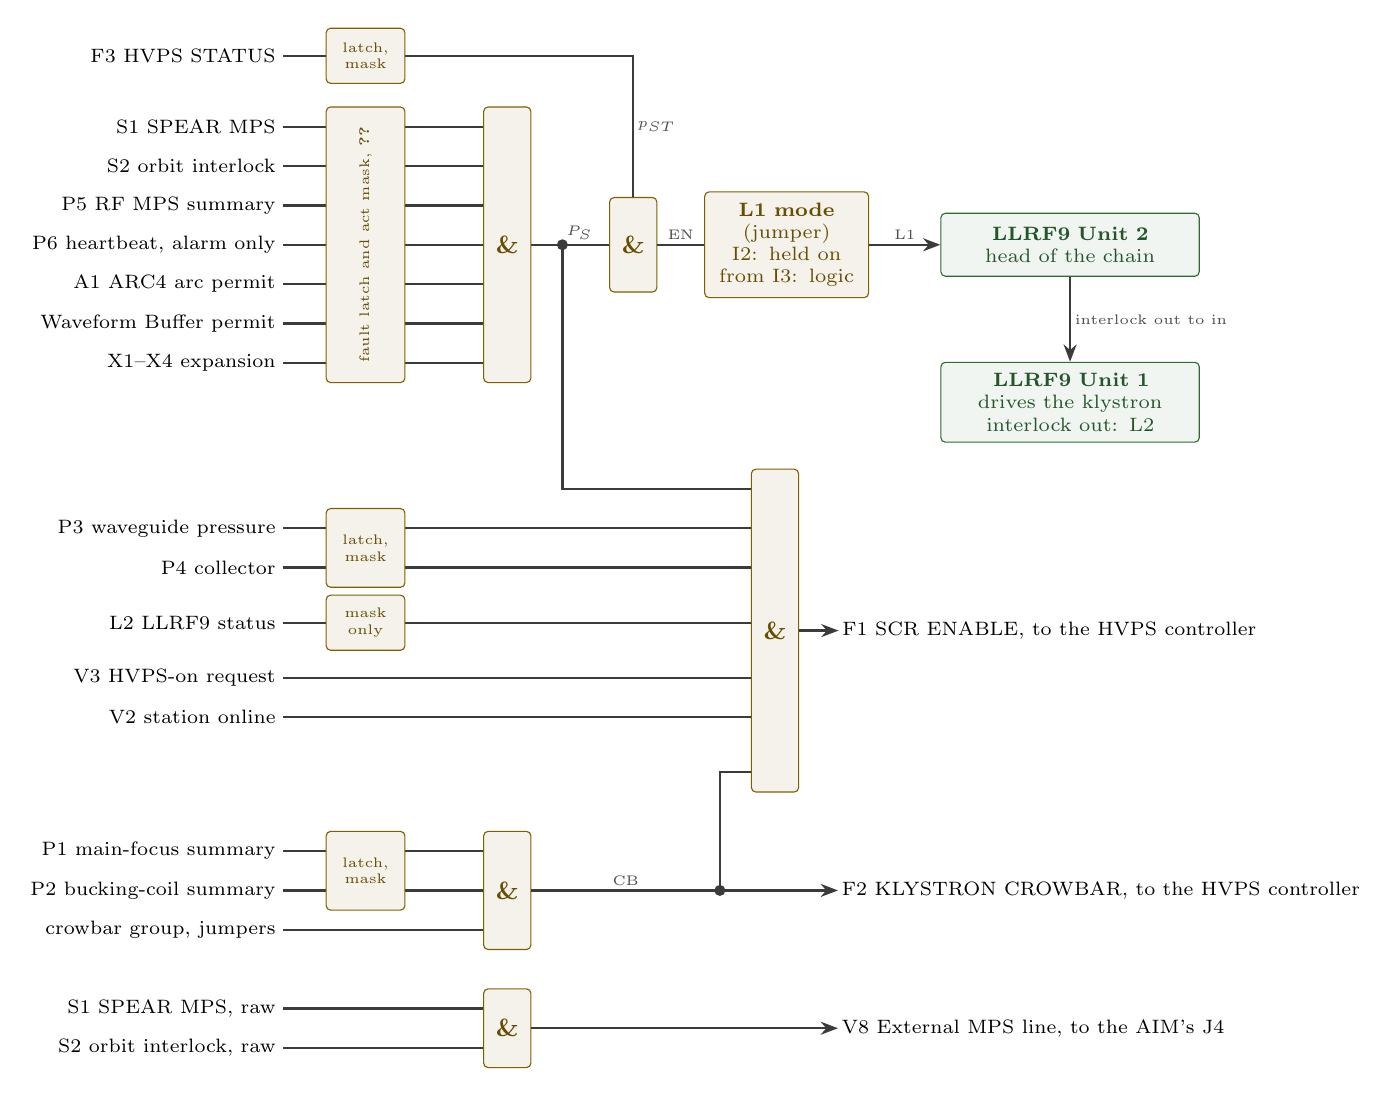
\begin{tikzpicture}[font=\scriptsize, x=1mm, y=1mm,
  every node/.append style={execute at begin node=\hyphenpenalty 10000\relax},
  il/.style={anchor=east,inner sep=1pt},
  ol/.style={anchor=west,inner sep=1pt},
  w/.style={draw=cNeut,thick},
  gate/.style={plc,minimum width=6mm,inner sep=0pt,font=\small\bfseries},
  lm/.style={plc,minimum width=10mm,inner sep=0pt,font=\tiny,align=center},
  dot/.style={circle,fill=cNeut,inner sep=0pt,minimum size=1.4mm}]

% ----- HVPS STATUS: latched, enters the LLRF9 enable only -------------------------
\node[il] at (30,9) {F3 HVPS STATUS};
\node[lm,minimum height=7mm] (lb) at (41,9) {latch,\\ mask};
\draw[w] (30.5,9) -- (lb.west);

% ----- station permits ---------------------------------------------------------
\foreach \y/\t in {0/S1 SPEAR MPS, -5/S2 orbit interlock, -10/P5 RF MPS summary,
                   -15/{P6 heartbeat, alarm only}, -20/A1 ARC4 arc permit,
                   -25/Waveform Buffer permit, -30/X1--X4 expansion}
  {\node[il] at (30,\y) {\t};
   \draw[w] (30.5,\y) -- (36,\y);
   \draw[w] (46,\y) -- (56,\y);}
\node[lm,minimum height=35mm] (la) at (41,-15) {};
\node[rotate=90,font=\tiny,text=cPlc!80!black] at (la) {fault latch and act mask, \cref{eq:pk}};
\node[gate,minimum height=35mm] (gps) at (59,-15) {\&};
\node[gate,minimum height=12mm] (gen) at (75,-15) {\&};
\draw[w] (gps.east) -- (gen.west) node[tag,pos=0.62,above]{$P_S$};
\draw[w] (lb.east) -- (lb.east -| gen.north) -- (gen.north);
\node[tag,right] at (75,0) {$p_{ST}$};

% ----- LLRF9 enable and the chain ------------------------------------------------
\node[plc,text width=18mm,anchor=west] (mode) at (84,-15)
  {\textbf{L1 mode} (jumper)\\ I2: held on\\ from I3: logic};
\draw[w] (gen.east) -- (mode.west) node[tag,midway,above]{EN};
\node[rf,text width=30mm,anchor=west] (u2) at (114,-15)
  {\textbf{LLRF9 Unit~2}\\ head of the chain};
\node[rf,text width=30mm,anchor=west] (u1) at (114,-35)
  {\textbf{LLRF9 Unit~1}\\ drives the klystron\\ interlock out: L2};
\draw[sig] (mode.east) -- (u2.west) node[tag,midway,above]{L1};
\draw[sig] (u2.south) -- (u2.south |- u1.north)
  node[tag,midway,right]{interlock out to in};

% ----- SCR ENABLE ----------------------------------------------------------------
\node[gate,minimum height=41mm] (gscr) at (93,-64) {\&};
\node[dot] at (66,-15) {};
\draw[w] (66,-15) |- (gscr.west |- 0,-46);
\foreach \y/\t in {-51/P3 waveguide pressure, -56/P4 collector}
  {\node[il] at (30,\y) {\t}; \draw[w] (30.5,\y) -- (36,\y); \draw[w] (46,\y) -- (90,\y);}
\node[lm,minimum height=10mm] at (41,-53.5) {latch,\\ mask};
\node[il] at (30,-63) {L2 LLRF9 status};
\draw[w] (30.5,-63) -- (36,-63); \draw[w] (46,-63) -- (90,-63);
\node[lm,minimum height=7mm] at (41,-63) {mask\\ only};
\foreach \y/\t in {-70/V3 HVPS-on request, -75/V2 station online}
  {\node[il] at (30,\y) {\t}; \draw[w] (30.5,\y) -- (90,\y);}
\draw[sig] (gscr.east) -- ++(5,0) node[ol]{F1 SCR ENABLE, to the HVPS controller};

% ----- KLYSTRON CROWBAR ----------------------------------------------------------
\foreach \y/\t in {-92/P1 main-focus summary, -97/P2 bucking-coil summary}
  {\node[il] at (30,\y) {\t}; \draw[w] (30.5,\y) -- (36,\y); \draw[w] (46,\y) -- (56,\y);}
\node[lm,minimum height=10mm] at (41,-94.5) {latch,\\ mask};
\node[il] at (30,-102) {crowbar group, jumpers};
\draw[w] (30.5,-102) -- (56,-102);
\node[gate,minimum height=15mm] (gcb) at (59,-97) {\&};
\node[dot] at (86,-97) {};
\draw[w] (86,-97) |- (gscr.west |- 0,-82);
\draw[w] (gcb.east) -- (86,-97) node[tag,midway,above]{CB};
\draw[sig] (86,-97) -- (101,-97) node[ol]{F2 KLYSTRON CROWBAR, to the HVPS controller};

% ----- External MPS line ---------------------------------------------------------
\foreach \y/\t in {-112/S1 SPEAR MPS{,} raw, -117/S2 orbit interlock{,} raw}
  {\node[il] at (30,\y) {\t}; \draw[w] (30.5,\y) -- (56,\y);}
\node[gate,minimum height=10mm] (gx) at (59,-114.5) {\&};
\draw[sig] (gx.east) -- (101,-114.5) node[ol]{V8 External MPS line, to the AIM's J4};
\end{tikzpicture}

\end{fitpicture}
\caption[Permit logic of the interlock board.]{Permit logic of the interlock board,
\crefrange{eq:station}{eq:xmps}. Every latched input passes its fault latch and act
mask, \cref{eq:pk}; the LLRF9 status L2 has only a mask in the permit path, because
the LLRF9 latches it itself; the commands V2 and V3 do not latch. The LLRF9 units are
daisy-chained outside the chassis: the enable L1 reaches Unit~1 through Unit~2, and
Unit~1's interlock output returns as the input L2. The External MPS
line V8 follows the raw machine permits.}\label{fig:logic}
\end{figure}

\subsection{Notation}

Every symbol in the equations is binary: 1 means a permit present, a request active or
an output on; $\wedge$ is AND, $\vee$ OR and $\neg$ NOT. Each permit input $k$ has
three states: $x_k = 1$ while its permit is present (\qty{24}{\volt} on the line, the
fiber lit or the LLRF9 output high), $a_k = 1$ when its act mask is set (LG-8), and
$L_k = 1$ while its fault latch is set. The latch is set when $x_k = 0$ and is cleared
by a reset only if $x_k = 1$ at that moment. The effective permit of the input is
\begin{equation}
p_k = \neg\,(a_k \wedge L_k), \label{eq:pk}
\end{equation}
so an input whose mask is off never removes a permit, while its latch still records
every fault. The LLRF9 status is latched inside the LLRF9 itself, so in the permit
path it acts without a chassis latch,
\[
q_u = \neg a_u \vee x_u,
\]
and has a record latch only (LG-6). Command inputs request an action and do not
latch. \Cref{tab:symbols} lists every symbol with its signal (\cref{tab:signals}) and
its source.

\begin{longtable}[c]{@{}Q{\cw{0.12}{1.5}}Q{\cw{0.44}{1.5}}Q{\cw{0.20}{1.5}}Q{\cw{0.24}{1.5}}@{}}
\caption{Symbols of the logic.}\label{tab:symbols}\\
\toprule
Symbol & Equal to 1 when & Signal & Source \\
\midrule
\endfirsthead
\toprule
Symbol & Equal to 1 when & Signal & Source \\
\midrule
\endhead
\bottomrule
\endlastfoot
$p_{MPS}$ & The RF MPS gives its summary permit, the global interlock sum (AB
summary) & P5 (J3-09) & PLC-5 O:031/0, then the ControlLogix \\
$p_{HB}$ & Heartbeat pulses arrive within the watchdog timeout (IC-10); its act mask
stays off, so it only alarms (D2) & P6 (J3-21) & PLC-5 O:031/5, then the
ControlLogix \\
$p_{SMPS}$ & The SPEAR MPS gives its beam permit & S1 & SPEAR MPS \\
$p_{ORB}$ & The orbit interlock gives its permit & S2 & Orbit interlock \\
$p_{ARC}$ & No arc & A1 & ARC4 system modules \\
$p_{WB}$ & No Waveform Buffer comparator or collector-power trip (WB-7) & Between the
boards & Waveform Buffer \\
$p_{X1}$ to $p_{X4}$ & Each assigned expansion permit present & X1 to X4 & As
assigned \\
$P_S$ & All ten permits above: the station permit, \cref{eq:station} & --- & --- \\
$p_{ST}$ & STATUS lit: the controller enabled by its PLC and no crowbar
trigger; the latched effective permit & F3 & HVPS
controller \\
$p_{FM}$ & Main-focus summary on: filament requested, main-focus voltage and current
inside their limits, supply's internal contact closed & P1 (J2-07) & PLC-5 output 032
(O:031/12) \\
$p_{BC}$ & Bucking-coil summary on: filament requested, bucking-coil voltage and
current inside their limits & P2 (J2-20) & PLC-5 output 033 (O:031/13) \\
$P_{CB}$ & Every further input assigned to the crowbar group by jumper gives its
permit; 1 when none is assigned, the default (D3) & Jumpers (LG-8) & --- \\
$p_{WGA}$ & Waveguide air-pressure summary on & P3 (J3-06) & PLC-5 O:030/12 \\
$p_{COL}$ & No collector-power trip: the PLC-5 latches one when the HVPS power less
the klystron output power stays above \qty{1200}{\kilo\watt} for \qty{0.7}{\second} &
P4 (J3-16) & PLC-5 O:031/6 \\
$q_u$ & LLRF9 status high: Unit~1's interlock output, high only while neither unit is
tripped and the enable is present & L2 & LLRF9 Unit~1 \\
$c_{HV}$ & HVPS on requested & V3 (J15 pin~2, HVPS\_ON) until I7; the chassis IOC
from I8 & State machine through the AIM, then the coordinator \\
$c_{ON}$ & Station online requested & V2 (J15 pin~14, SOLENOID\_ON) until I7; the
chassis IOC from I8 & Operator through EPICS and the AIM, then the coordinator \\
$\sig{EN}$ & LLRF9 enable on & L1 & To Unit~2's interlock input \\
$\sig{CB}$ & KLYSTRON CROWBAR lit: no crowbar & F2 & To the HVPS controller \\
$\sig{SCR}$ & SCR ENABLE lit: triggers enabled & F1 & To the HVPS controller \\
$\sig{XMPS}$ & External MPS line held low: both machine permits present & V8 & To
the AIM's J4, I2 to I7 \\
\end{longtable}

\subsection{Equations}

The station permit is the product of every permit that must stop the RF:
\begin{equation}
P_S = p_{MPS} \wedge p_{HB} \wedge p_{SMPS} \wedge p_{ORB} \wedge p_{ARC} \wedge p_{WB}
\wedge p_{X1} \wedge p_{X2} \wedge p_{X3} \wedge p_{X4}. \label{eq:station}
\end{equation}
The outputs are:
\begin{align}
\sig{EN} &= P_S \wedge p_{ST}, \label{eq:en}\\
\sig{CB} &= p_{FM} \wedge p_{BC} \wedge P_{CB}, \label{eq:cb}\\
\sig{SCR} &= c_{HV} \wedge c_{ON} \wedge \sig{CB} \wedge p_{WGA} \wedge p_{COL}
\wedge P_S \wedge q_{u}, \label{eq:scr}\\
\sig{XMPS} &= x_{SMPS} \wedge x_{ORB}. \label{eq:xmps}
\end{align}
An input whose act mask is off drops out of every equation but \cref{eq:xmps}
(\cref{eq:pk} and $q_u$); \cref{tab:phases} gives when each input acts, and
\cref{tab:logic-why} the reason for each term. \Cref{fig:logic} draws the equations.

\begin{longtable}[c]{@{}Q{\cw{0.16}{1.333}}Q{\cw{0.54}{1.333}}Q{\cw{0.30}{1.333}}@{}}
\caption{Reasons for each term.}\label{tab:logic-why}\\
\toprule
Output & Term and reason & Basis \\
\midrule
\endfirsthead
\toprule
Output & Term and reason & Basis \\
\midrule
\endhead
\bottomrule
\endlastfoot
LLRF9 enable & Every station permit removes the drive: the RF MPS, the SPEAR MPS, the
orbit interlock, an arc, a Waveform Buffer trip and the HVPS STATUS,
which goes dark when the crowbar fires or the controller's PLC stops (IC-4) & \R{4},
\R{8} \\
LLRF9 enable & No dependence on SCR ENABLE or on the LLRF9 status, so that the units
can be reset while the HVPS is off and no permit waits on itself. A trip of Unit~2,
such as on reflected power, reaches the drive of Unit~1 through the daisy chain, not
through the chassis (D1) & \R{1}, \R{4}, \R{20} \\
KLYSTRON CROWBAR & Fired, and latched, on a main-focus or bucking-coil summary fault:
a coil current outside its limits can steer the beam into the tube body, as the panel
does today. & \R{9}, \R{11}, \R{12},
\R{13} \\
SCR ENABLE & The HVPS-on request and the waveguide air-pressure and collector-power
summaries, as in the panel; the station-online command in place of the panel's online
key, so that taking the station offline from EPICS removes SCR ENABLE at once (D6) &
\R{11}, \R{13} \\
SCR ENABLE & Dark whenever KLYSTRON CROWBAR is dark, as a redundant inhibit & \R{9} \\
SCR ENABLE & Every station permit, and from I6 the LLRF9 status (D12): with the drive
off the collector would take the full beam power & \R{4},
\R{8}, \R{11} \\
SCR ENABLE & The RF MPS summary permit from I2, which the panel did not use: every RF
MPS trip already trips the station through the AIM, and the chassis now removes the
high voltage at once instead of after the state machine's ramp-down (D2) & \R{19},
\R{23} \\
None & The RF MPS heartbeat only alarms, as on the AIM today; a stopped RF MPS removes
the summary permit if its outputs turn off (D2, O9) & \R{19}, \R{23} \\
SCR ENABLE & Not the HVPS STATUS: a dark STATUS means that the controller has already
inhibited its triggers or fired the crowbar; from I3 STATUS removes the LLRF9 enable,
and from I6, through the LLRF9 status, SCR ENABLE & \R{4}, \R{8}, \R{10} \\
External MPS line & The raw permits, from I2, before the masks are set: the AIM
latches, reports and resets the channel as it does with Slot~5's J3, and the legacy
software needs no change & \R{2}, \R{23} \\
\end{longtable}

Expected, and compared with the baseline of the panel: with the filament off the coil
summaries are off, so KLYSTRON CROWBAR stays dark and latched until the reset of the
next turn-on.

\subsection{Latching, Reset and First Fault}\label{sec:logic-reset}

\begin{longtable}[c]{@{}Q{\cw{0.08}{1.333}}Q{\cw{0.70}{1.333}}Q{\cw{0.22}{1.333}}@{}}
\caption{Latching, reset and first-fault requirements.}\label{tab:req-latch}\\
\toprule
ID & Requirement & Basis \\
\midrule
\endfirsthead
\toprule
ID & Requirement & Basis \\
\midrule
\endhead
\bottomrule
\endlastfoot
LG-1 & Every permit input has a fault latch, set by the input whatever its act mask,
and cleared only by a reset while the input is healthy. & \R{4} \\
LG-2 & A reset acts on its rising edge and resets all latches at once. It comes from
FAULT\_RESET on J15 (I2 to I7) or an EPICS command through the chassis IOC, and is
passed on to the RF MPS on P10 (IC-11);
there is no front-panel reset (IC-38). A reset line held active does not hold the latches
clear; a reset held for more than \qty{10}{\second} is reported (\emph{proposed}). &
\R{1}, \R{4} \\
LG-3 & The crowbar latch is cleared by the same reset, which also resets the ARC4
latch and the Waveform Buffer comparators. & \R{1}, \R{13} \\
LG-4 & A first-fault register captures the latches of all acting inputs at the first
fault after a reset and holds them until the next reset. Faults closer together than
\qty{100}{\nano\second} are recorded together (\emph{proposed}). & \R{1}, \R{4} \\
LG-5 & A second register does the same for inputs whose act mask is off, so that a
monitor-only run records what would have tripped. & \R{3} \\
LG-6 & The LLRF9 status has a record latch and enters both registers, although it
acts directly in the permit path. & \R{4} \\
LG-7 & A fault that a removed output causes, such as an LLRF9 trip after its enable was
removed, does not displace the first fault. & \R{4} \\
\end{longtable}

\subsection{Act Masks}

\begin{longtable}[c]{@{}Q{\cw{0.08}{1.333}}Q{\cw{0.70}{1.333}}Q{\cw{0.22}{1.333}}@{}}
\caption{Act mask requirements.}\label{tab:req-mask}\\
\toprule
ID & Requirement & Basis \\
\midrule
\endfirsthead
\toprule
ID & Requirement & Basis \\
\midrule
\endhead
\bottomrule
\endlastfoot
LG-8 & One act mask per permit input, the crowbar-group selection of each input, the
mode of the LLRF9 enable (held on or by the logic, IC-5) and the J15 or IOC command
source are set by
jumpers or switches inside the chassis, never by software. & \R{3}, \R{4} \\
LG-9 & Every mask is read back, shown on the front panel when off and reported to
EPICS, so that the configuration of each integration is recorded. & \R{3} \\
LG-10 & The masks follow \cref{tab:phases}; the configuration of each integration is
part of its entry criteria. & \R{3} \\
\end{longtable}

% ===========================================================================
\section{Station Shut-Off and Reset}\label{sec:shutoff}

This section sets out how the station shuts off and how it is reset and turned on
again, today and with the chassis from I2. It is read from the state machine, the
station records and the programs of the RF MPS and the HVPS controller \R{19}, \R{22},
\R{23}, \R{27}; where the behavior rests on logic that is not documented, the panel's
equations and the AIM's commands, it is marked (O1, O4).

\subsection{Latches and Resets}

\Cref{tab:latches} lists each unit that latches a trip and what resets it.

\begin{longtable}[c]{@{}Q{\cw{0.16}{1.5}}Q{\cw{0.24}{1.5}}Q{\cw{0.32}{1.5}}Q{\cw{0.28}{1.5}}@{}}
\caption{Latches of the station and their resets.}\label{tab:latches}\\
\toprule
Unit & Latches & Reset today & From I2 \\
\midrule
\endfirsthead
\toprule
Unit & Latches & Reset today & From I2 \\
\midrule
\endhead
\bottomrule
\endlastfoot
AIM (VXI slot~12) & Its arc channels, the VXI backplane fault (any RF\_FAULT), the AB
summary and heartbeat, the forced fault, External MPS and the beam abort \R{23} &
\fpath{SRF1:STN:AIM:MODU.RSTF}, which also sends FAULT\_RESET on J15: three times in
the reset sequence, once at the end of each turn-on and many times in its
arc-threshold test \R{22}, \R{23}. A forced fault holds until an operator turns it off
& Unchanged, with its arc channels quiet (IC-27c); each FAULT\_RESET also resets the
chassis. Retired at I8 \\
Panel, then interlock board & The panel: the crowbar and the beam abort, in two
flip-flops \R{13} & FAULT\_RESET through the Fast Interlock Chassis, which the panel
passes on to the PLC-5 (J2-23) \R{12}, \R{13} & Every permit input (LG-1), reset by
FAULT\_RESET until I7, by the chassis IOC (ST-4) and from I8 by the coordinator; passed
on to the RF MPS (P10) and followed by the LLRF9 resets (ST-8) \\
RF MPS (PLC-5; \mbox{ControlLogix} from I4) & Each fault, and the summaries that it drops,
the AB summary (P5) among them \R{19} & Its reset line I:030/0, from the panel: while
the line is high each latch whose fault has cleared is released, and the summaries
return at the end of that scan \R{19} & The same line, P10, driven by the chassis
(RS-1) \\
HVPS controller (SLC-500 in B118) & Its own faults, such as the crowbar, the arcs and
an overvoltage, and the SCR ON latch that runs its regulator \R{23}, \R{27} &
\fpath{SRF1:HVPS:RESET:CTRL} over Remote I/O, in the reset sequence, or its local
reset; never through the fibers. The SCR ON latch sets only within
\qty{0.5}{\second} of the trigger enable \fpath{SRF1:HVPSSCR:ON:CTRL} turning on, and
only with SCR ENABLE lit \R{23}, \R{27} & Unchanged until I7 \\
RFP and IQAs (VXI) & Their RF faults, which drive RF\_FAULT \R{23} & Fault and latch
resets in the reset sequence \R{23} & Unchanged until I8 \\
LLRF9 Units~1 and 2 & The interlock input and the internal trips of each unit \R{20}
& By hand, \texttt{\$(SYS):\allowbreak{}ILOCK:\allowbreak{}RESET} of each unit, while
they are monitor-only (I1) \R{26} & By the chassis IOC after each chassis reset,
Unit~2 then Unit~1 (ST-8) \\
ARC4 & The fired detector (O3) & None: monitor-only from I1 & The chassis reset
(LG-3) \\
\end{longtable}

\subsection{Shut-Off}

Today every trip ends in the state machine's turn-off \R{22}. Once a station summary
turns bad (\fpath{SRF1:STNOFF:SUMY:STAT}) the state machine forces the beam abort and,
after \qty{1}{\second}, sets the RFP to TUNE; sets the HVPS voltage request to zero
and waits \qty{5}{\second}; turns off the HVPS trigger enable over Remote I/O, the RF
switch and the loops; and, after a fault, saves the fault files. The trigger enable
stops the regulator of the HVPS controller, whose SCR ON latch drops, but leaves the
contactor closed, so STATUS stays lit (\cref{sec:io-hvps}) \R{27}. A dark SCR ENABLE
stops the triggers at once, in hardware; the controller's program then drops the same
latch, which the state machine reads as a lost supply-on status
(\fpath{SRF1:HVPSSUPPLY:ON:STAT}) and answers with the same turn-off \R{23}, \R{27}.
\Cref{tab:shutoff} follows each trip.

\begin{longtable}[c]{@{}Q{\cw{0.20}{1.333}}Q{\cw{0.42}{1.333}}Q{\cw{0.38}{1.333}}@{}}
\caption{Shut-off by trip.}\label{tab:shutoff}\\
\toprule
Trip & Today & From I2 \\
\midrule
\endfirsthead
\toprule
Trip & Today & From I2 \\
\midrule
\endhead
\bottomrule
\endlastfoot
RF fault in the VXI crate: RFP, IQA, AIM, forced fault & RF\_FAULT zeroes the drive at
once; the turn-off ramps the high voltage down and ends it after about
\qty{6}{\second}, unless the panel or the AIM removes it earlier through logic that is
not documented (O1, O4) \R{22}, \R{23} & As today; the chassis sees the trip only if the AIM drops its
HVPS-on request ($c_{HV}$), and the IOC freezes the Waveform Buffer (ST-9). From I6
the LLRF9 drives, and its trips remove SCR ENABLE (D12) \\
SPEAR MPS or orbit permit & Slot~5 asserts RF\_FAULT and the AIM's External MPS; then
as above, or the PLC-5's collector protection removes SCR ENABLE through the panel
after \qty{0.7}{\second} if the collector power stays above \qty{1200}{\kilo\watt}
\R{2}, \R{19} & Also latched in the chassis and, once acting, SCR
ENABLE dark at once; External MPS driven by the chassis (IC-27b); from I3 the LLRF9
enable removed \\
RF MPS trip (AB summary) & The AIM latches it and asserts RF\_FAULT; then as above
\R{19}, \R{23} & SCR ENABLE dark at once, latched (P5, D2); the AIM path unchanged \\
Collector-power or waveguide air-pressure summary & The panel removes SCR ENABLE at
once; the AB summary trips too \R{13}, \R{19} & As today, and latched in the chassis \\
Main-focus or bucking-coil summary & The panel darkens KLYSTRON CROWBAR, latched, and
SCR ENABLE: the controller fires the crowbar and inhibits its triggers; its program
then drops the SCR ON latch and opens the contactor, unless its crowbar-lockout bit is
set, so STATUS stays dark until the contactor is closed again and the station turns
off with no automatic reset \R{10}, \R{13}, \R{27} & As
today, by \cref{eq:cb}; the dark STATUS latches F3, which from I3 removes the LLRF9
enable \\
HVPS controller: arc trigger or own fault & The controller fires the crowbar or
inhibits its triggers itself and drops its SCR ON latch; after a crowbar or a current
trip it also opens the contactor, so STATUS stays dark until the contactor is closed
again; the station turns off on the HVPS summaries, with no automatic reset while the
contactor is open \R{10}, \R{23}, \R{27} & As today; F3 latched, a record at I2; from
I3 it removes the LLRF9 enable, and from I6, through the LLRF9 status, SCR ENABLE \\
ARC4 or Waveform Buffer trip & None & Latched; once acting, SCR ENABLE dark at once,
and the station turns off on the lost supply-on status; the IOC records the cause
(ST-3, ST-7) \\
Operator turn-off & The turn-off, with no fault files and no automatic reset; STATUS
stays lit \R{22}, \R{27} & As today; no chassis latch is set, so from I3 the LLRF9
enable stays on \\
Station offline (\fpath{SRF1:STN:AIM:SOLENOID}) & The PLC-5's online bit drops
(\fpath{SRF1:STN:LOCAL:ON}) and the station turns off, with no automatic reset; the
panel's SCR ENABLE follows its key switch instead \R{13}, \R{22} & SCR ENABLE dark at
once ($c_{ON}$, D6); then as today \\
HVPS contactor opened, by an operator or on a heater fault & STATUS goes dark; the
station turns off on the HVPS summaries, with no automatic reset while the contactor
is open \R{22}, \R{27} & F3 latched: from I3 the LLRF9 enable stays off until a reset
after the contactor closes again \\
Chassis power or IOC lost & --- & Power: every permit removed and the crowbar fired
(IC-42); a reset is needed after power returns (IC-43). IOC: no permit changes, but no
LLRF9 resets (ST-8), so from I3 a tripped LLRF9 is reset from its own screens \\
\end{longtable}

\subsection{Reset and Restart}

\paragraph{Reset sequence.} An operator resets the station with
\fpath{SRF1:STN:RESET:CTRL}, which runs for about \qty{3.2}{\second} \R{23}:
\begin{itemize}
\item at \qty{0}{\second}, the IQA faults cleared;
\item at \qty{0.1}{\second}, the AIM reset; its FAULT\_RESET resets the panel, from I2
the chassis, and through J2-23 (P10) the PLC-5;
\item at \qty{0.2}{\second}, the RFP and IQA latches reset, and the HVPS controller
reset started on \fpath{SRF1:HVPS:RESET:CTRL} over Remote I/O;
\item at \qty{2.2}{\second}, the AIM and the RFP reset again, and the HVPS reset ended:
the record makes a \qty{3}{\second} pulse, but the sequence writes it back to zero;
\item at \qty{3.2}{\second}, the AIM reset a third time.
\end{itemize}
The later AIM resets clear what the first cannot. The PLC-5 releases its latches only
while its reset line is high and sets its summaries at the end of that scan, so at the
first reset the AIM's latch of the AB summary, and from I2 the chassis latch of P5,
still sees the fault; they clear at the second \R{19}, \R{23}.

\paragraph{Automatic reset.} After a turn-off on a fault the state machine resets the
station by itself if the retry count \fpath{SRF1:STN:RESET:COUNTER} is above zero, no
forced fault is set and the HVPS contactor is closed with the station online. It runs
the reset sequence, lowers the count by one and waits \qty{5}{\second}, until the
turn-on summary (\fpath{SRF1:STNON:SUMY:STAT}) is clean or the count runs out; then it
turns the station back on in the state it had, or leaves it off \R{22}. Either an accepted procedure for this or a summary record the legacy summary can read.

\paragraph{Turn-on.} The turn-on to ON\_CW spends four to five seconds loading the
DACs, homing the tuners and setting the loops; it then turns on the RF switch, sets
the HVPS voltage request, and gives the trigger enable over Remote I/O and the HVPS-on
request through the AIM together. Once the station is up it resets the beam abort
and, through the AIM, the faults once more \R{22}. The HVPS controller sets its
SCR ON latch only within \qty{0.5}{\second} of the trigger enable and only while SCR
ENABLE is lit \R{27}: a SCR ENABLE that lights later does not start the HVPS until the
next turn-on.

\paragraph{From I2.} The chassis takes each of these resets from FAULT\_RESET, as the
panel did, and the IOC follows each with the LLRF9 resets (ST-8), so the legacy
sequences need no change. Until I8 operators reset with the legacy sequence, which
also resets the AIM; a reset from the chassis IOC clears only the chassis and, through
P10, the RF MPS. From I3 the LLRF9 trips whenever the chassis removes its enable; by
\cref{eq:en} the enable returns once the station permits and STATUS are healthy and
reset, whatever SCR ENABLE and the LLRF9 units show, so no permit waits on itself
\R{4}, \R{10}. \Cref{tab:req-reset} sets the rules that the sequences rely on.

\begin{longtable}[c]{@{}Q{\cw{0.08}{1.333}}Q{\cw{0.70}{1.333}}Q{\cw{0.22}{1.333}}@{}}
\caption{Reset requirements.}\label{tab:req-reset}\\
\toprule
ID & Requirement & Basis \\
\midrule
\endfirsthead
\toprule
ID & Requirement & Basis \\
\midrule
\endhead
\bottomrule
\endlastfoot
RS-1 & Every reset reaches the RF MPS on P10 as a pulse of at least
\qty{100}{\milli\second} (\emph{proposed}), however short the request, so that the
PLC-5, and from I4 the \mbox{ControlLogix}, sees it within a scan. & \R{19} \\
RS-2 & A reset releases a latch only while its input is healthy (LG-1), so a latch of
an RF MPS line that the same reset clears in the RF MPS, such as P5, releases at a
later reset. The legacy sequence gives three resets; a reset from the chassis IOC
(ST-4), and from I8 from the coordinator, is repeated once about \qty{2}{\second}
later (\emph{proposed}), each followed by the LLRF9 resets. & \R{19}, \R{23} \\
RS-3 & A restart keeps this order: the fault cleared; the HVPS contactor closed, with
STATUS lit; the resets of the chassis, the RF MPS, the HVPS controller and the AIM;
the LLRF9 resets, Unit~2 before Unit~1, because Unit~1's input waits on Unit~2's
output; then the turn-on, with SCR ENABLE lit within \qty{0.5}{\second} of the trigger
enable. STATUS goes dark whenever the contactor opens, so a reset follows each
closing. The legacy automatic reset keeps this order; from I8 the coordinator keeps it
and checks SCR ENABLE before it gives the trigger enable. & \R{4}, \R{22}, \R{27} \\
RS-4 & A reset while the station runs, such as the one at the end of each turn-on,
changes no output, and the LLRF9 resets that follow it leave a running unit
undisturbed. & \R{22}, \R{26} \\
\end{longtable}

The legacy turn-on summary does not include the chassis latches: a latch that the
resets cannot clear lets the automatic reset turn the station on without high voltage,
until its retry count runs out \R{22}, \R{23}. 

% ===========================================================================
\section{Electrical, Timing and Fail-Safe Requirements}\label{sec:electrical}

\begin{longtable}[c]{@{}Q{\cw{0.16}{1.333}}Q{\cw{0.62}{1.333}}Q{\cw{0.22}{1.333}}@{}}
\caption{Electrical classes.}\label{tab:classes}\\
\toprule
Class & Requirement & Basis \\
\midrule
\endfirsthead
\toprule
Class & Requirement & Basis \\
\midrule
\endhead
\bottomrule
\endlastfoot
\qty{24}{\volt} in & Isolated by an optocoupler such as the Broadcom ACSL-6xx0 family
(about \qty{50}{\nano\second}), with a series resistor sized for
\qtyrange{7}{10}{\milli\ampere} at \qty{24}{\volt} (\qty{2.2}{\kilo\ohm} to
\qty{2.8}{\kilo\ohm}) unless a lower current is required (IC-13). On above
\qty{15}{\volt}, off below \qty{5}{\volt}; off with up to \qty{1}{\milli\ampere}
leakage from a PLC output; withstands \qty{35}{\volt} and reverse polarity
(\emph{proposed} levels). & \R{4}, \R{7}, \R{8} \\
TTL in & Isolated Schmitt-trigger input, threshold \qtyrange{1.2}{2.0}{\volt},
withstands \qty{\pm 15}{\volt} (\emph{proposed}). AIM inputs (V1 to V5): a
\qty{2}{\kilo\ohm} pull-up to \qty{5}{\volt}, as on the Fast Interlock Chassis
(IC-25); expansion inputs (X1, X2): about \qty{1}{\kilo\ohm} to ground (IC-21). &
\R{4}, \R{14} \\
LLRF9 in & As IC-6. & \R{20} \\
Fiber in, out & As IC-1 and IC-2. & \R{8} \\
\qty{24}{\volt} out & Isolated sourcing output, at least \qty{20}{\volt} at
\qty{20}{\milli\ampere}, leakage at most \qty{0.5}{\milli\ampere} when off,
short-circuit protected (\emph{proposed}); able to drive the 1771-IBN and its
ControlLogix replacement. & \R{18} \\
LLRF9 out & As IC-5. & \R{20} \\
TTL out & Isolated open-collector output with a \qty{1}{\kilo\ohm} pull-up to
\qty{5}{\volt}, low at most \qty{0.5}{\volt} while sinking \qty{8}{\milli\ampere}
(\emph{proposed}); drives the AIM's \qty{10}{\kilo\ohm} inputs, and on pin~10 its
\qty{1}{\micro\farad}, as the Fast Interlock Chassis does (IC-25). & \R{14}, \R{15} \\
Switch out & As IC-27b. & \R{15} \\
\end{longtable}

\begin{longtable}[c]{@{}Q{\cw{0.08}{1.333}}Q{\cw{0.70}{1.333}}Q{\cw{0.22}{1.333}}@{}}
\caption{Isolation, timing and fail-safe requirements.}\label{tab:req-elec}\\
\toprule
ID & Requirement & Basis \\
\midrule
\endfirsthead
\toprule
ID & Requirement & Basis \\
\midrule
\endhead
\bottomrule
\endlastfoot
IC-39 & Every electrical input and output is isolated from the chassis logic and from
every other connector group, by optocoupler, digital isolator or relay; at least
\qty{1.5}{\kilo\volt} rms (\emph{proposed}). The returns of external signals are not
tied to the chassis logic ground. & \R{1}, \R{4} \\
IC-40 & Propagation from a change of any fiber, LLRF9, SPEAR MPS, orbit, ARC4,
Waveform Buffer or TTL input to every output it affects: at most
\qty{5}{\micro\second} (\emph{proposed}); inputs from PLC lines add the filter of
IC-41. & \R{1}, \R{4} \\
IC-41 & Inputs from PLC lines may be filtered for up to \qty{1}{\milli\second}
against contact and switching noise (\emph{proposed}); other inputs reject pulses
shorter than \qty{1}{\micro\second} (\emph{proposed}). & --- \\
IC-42 & Loss of chassis power, of any internal supply or of the interlock
board removes every permit: both fibers dark, the LLRF9 enable low, the External MPS
line open. A dark KLYSTRON CROWBAR fiber fires the
crowbar, as with the panel today. & \R{1}, \R{10} \\
IC-43 & A supply monitor holds every permit off until all internal supplies are in
range and the logic is configured, and the latches come up set, so that a reset is
needed after power-up. & \R{4} \\
IC-44 & Faults of the chassis itself, such as a failed supply or a configuration
error, are latched and reported as their own first-fault entry. & --- \\
\end{longtable}

\Cref{tab:failsafe} gives the state the chassis takes for each failure of a partner.

\begin{longtable}[c]{@{}Q{\cw{0.30}{1.333}}Q{\cw{0.35}{1.333}}Q{\cw{0.35}{1.333}}@{}}
\caption{Fail-safe states.}\label{tab:failsafe}\\
\toprule
Failure & Seen by the chassis as & Result \\
\midrule
\endfirsthead
\toprule
Failure & Seen by the chassis as & Result \\
\midrule
\endhead
\bottomrule
\endlastfoot
Chassis power lost & --- & All permits removed (IC-42) \\
LLRF9 unit unpowered & LLRF9 status low, through the chain for either unit & SCR
ENABLE dark, from I6; Unit~1's drive stopped by the chain \\
HVPS controller off, its PLC stopped or crowbar fired & STATUS dark & The controller
inhibits its own triggers; from I3 the LLRF9 enable removed, latched, and from I6
with it SCR ENABLE \\
RF MPS stops & Summary permit lost if its outputs turn off (O9); heartbeat lost & SCR
ENABLE removed, latched, and from I3 the LLRF9 enable; a lost heartbeat alone raises a
MAJOR alarm (D2) \\
Cable to the SPEAR MPS or orbit interlock cut & Permit lost & External MPS on the
AIM at once; SCR ENABLE removed, latched, once the permits act (after I2), and from
I3 the LLRF9 enable \\
ARC4 unpowered or cable cut & Arc permit lost & As above, once the ARC4 acts \\
Waveform Buffer board fault & Its permit lost & As above, once it acts \\
37-pin cable to the AIM unplugged & --- & The AIM reads External MPS and its arc
inputs float, as with the Fast Interlock Chassis unplugged today \\
Network or IOC lost & Nothing & No permit changes; status and waveforms unavailable \\
\end{longtable}

% ===========================================================================
\section{Waveform Buffer}\label{sec:wfb}

The legacy IQAs digitize 24 detected RF signals at about 1~MSPS into 32-kilosample
circular buffers that freeze on a fault; the two LLRF9 units take the 18 most
important, and the Waveform Buffer takes the other six and the four HVPS signals of
the B118 oscilloscope, which triggers on a loss of HVPS voltage: the HVPS voltage and
current, the transformer current and the SCR firing signal, on its channels 1 to 4
\R{25}. The voltage and current also reach B132 through the HVPS monitor board \R{2};
the other two are taken in B118 (O8). On HVPS1 they are one phase current of
transformer~1 and the voltage on inductor~2, which shows the firing of transformer~2 \R{5}. An HVPS
failure has been seen to start about \qty{100}{\milli\second} before the trip \R{5}.
\Cref{fig:wfb} shows the signal paths on the board.

\begin{figure}[tbp]
\centering
\begin{fitpicture}
% !TeX root = ../C_interface_chassis_requirements.tex
% Waveform Buffer board: each conditioned signal goes to a digitizer and buffer
% and to a latched comparator; the latched trips form the WB permit. RF trips go
% up and HVPS trips down so that no path crosses another.
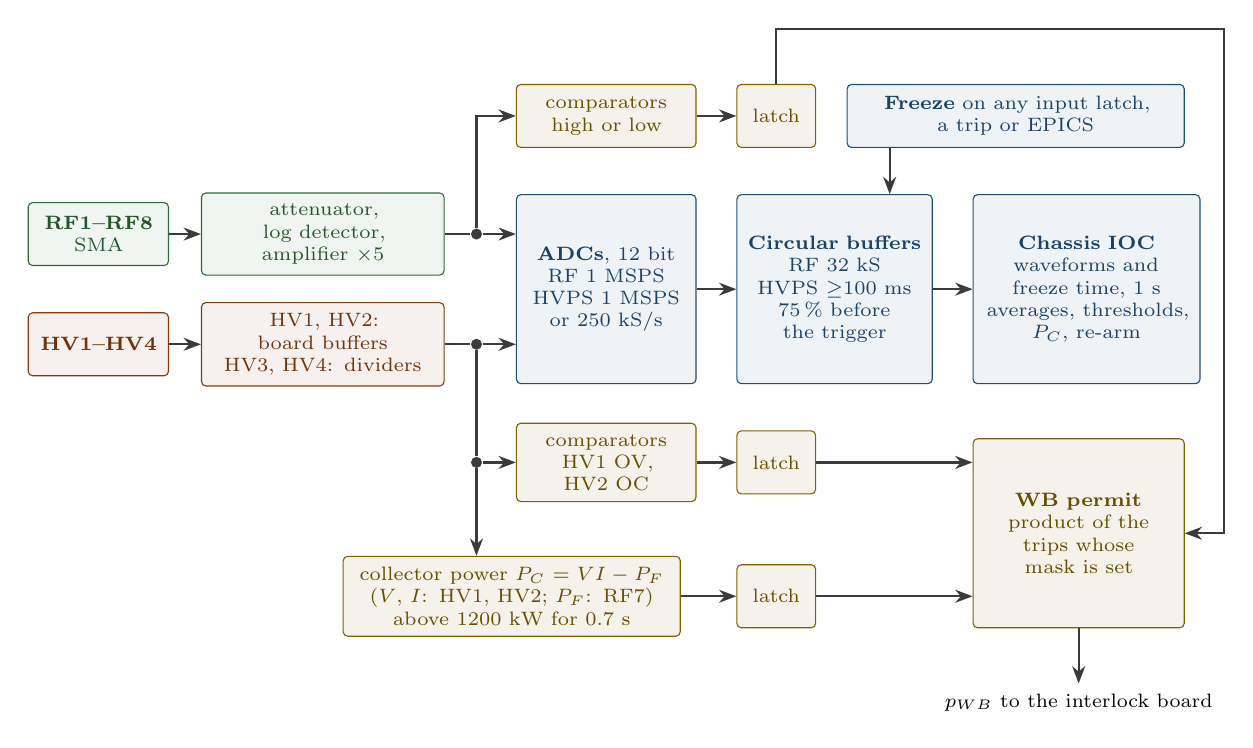
\begin{tikzpicture}[font=\scriptsize, x=1mm, y=1mm,
  every node/.append style={execute at begin node=\hyphenpenalty 10000\relax},
  w/.style={draw=cNeut,thick},
  dot/.style={circle,fill=cNeut,inner sep=0pt,minimum size=1.4mm}]

% ----- inputs and conditioning ---------------------------------------------------
\node[rf,text width=15mm,anchor=west]  (rfin) at (0,4)   {\textbf{RF1--RF8}\\ SMA};
\node[pwr,text width=15mm,anchor=west] (hvin) at (0,-10) {\textbf{HV1--HV4}};
\node[rf,text width=28mm,anchor=west]  (crf)  at (22,4)
  {attenuator, log detector,\\ amplifier ${\times}5$};
\node[pwr,text width=28mm,anchor=west] (chv)  at (22,-10)
  {HV1, HV2: board buffers\\ HV3, HV4: dividers};
\draw[sig] (rfin) -- (crf);
\draw[sig] (hvin) -- (chv);

% ----- digitizers, buffers and the IOC -------------------------------------------
\node[ctrl,text width=20mm,minimum height=24mm,anchor=west] (adc) at (62,-3)
  {\textbf{ADCs}, 12 bit\\ RF 1~MSPS\\ HVPS 1~MSPS\\ or 250~kS/s};
\node[ctrl,text width=22mm,minimum height=24mm,anchor=west] (buf) at (90,-3)
  {\textbf{Circular buffers}\\ RF 32~kS\\ HVPS $\geq$100~ms\\ 75\,\% before the trigger};
\node[ctrl,text width=26mm,minimum height=24mm,anchor=west] (ioc) at (120,-3)
  {\textbf{Chassis IOC}\\ waveforms and freeze time, 1~s averages, thresholds, $P_C$, re-arm};
\node[dot] (srf) at (57,4) {};
\node[dot] (shv) at (57,-10) {};
\draw[w] (crf.east) -- (srf);
\draw[w] (chv.east) -- (shv);
\draw[sig] (srf) -- (adc.west |- srf);
\draw[sig] (shv) -- (adc.west |- shv);
\draw[sig] (adc) -- (buf);
\draw[sig] (buf) -- (ioc);

% ----- freeze --------------------------------------------------------------------
\node[ctrl,text width=40mm,anchor=west] (frz) at (104,19)
  {\textbf{Freeze} on any input latch,\\ a trip or EPICS};
\draw[sig] ([xshift=-16mm]frz.south) -- ([xshift=-16mm]frz.south |- buf.north);

% ----- comparators and trips -----------------------------------------------------
\node[plc,text width=20mm,anchor=west] (cmr) at (62,19) {comparators\\ high or low};
\node[plc,anchor=west,minimum width=10mm] (lr) at (90,19) {latch};
\draw[sig] (srf) |- (cmr.west);
\draw[sig] (cmr) -- (lr);
\node[plc,text width=20mm,anchor=west] (cmh) at (62,-25) {comparators\\ HV1 OV, HV2 OC};
\node[plc,anchor=west,minimum width=10mm] (lh) at (90,-25) {latch};
\node[dot] (sh2) at (57,-25) {};
\draw[w] (shv) -- (sh2);
\draw[sig] (sh2) -- (cmh.west);
\draw[sig] (cmh) -- (lh);
\node[plc,text width=40mm,anchor=west] (pc) at (40,-42)
  {collector power $P_C = VI - P_F$\\ ($V$, $I$: HV1, HV2; $P_F$: RF7)\\ above 1200~kW for 0.7~s};
\node[plc,anchor=west,minimum width=10mm] (lp) at (90,-42) {latch};
\draw[sig] (sh2) -- (sh2 |- pc.north);
\draw[sig] (pc) -- (lp);

% ----- Waveform Buffer permit ----------------------------------------------------
\node[plc,text width=24mm,minimum height=24mm,anchor=west] (perm) at (120,-34)
  {\textbf{WB permit}\\ product of the trips whose mask is set};
\draw[sig] (lh.east) -- (perm.west |- lh.east);
\draw[sig] (lp.east) -- (perm.west |- lp.east);
\draw[sig] (lr.north) -- ++(0,7) -| ([xshift=5mm]perm.east) -- (perm.east);
\draw[sig] (perm.south) -- ++(0,-7) node[below]{$p_{WB}$ to the interlock board};
\end{tikzpicture}

\end{fitpicture}
\caption[Signal paths of the Waveform Buffer board.]{Signal paths of the Waveform
Buffer board. Each conditioned signal goes to a digitizer and a circular buffer, and
to a comparator whose latched trip, with the collector-power trip, forms the Waveform
Buffer permit to the interlock board (WB-7). The buffers freeze together on the
first latch of any input of the interlock board, a Waveform Buffer trip or an EPICS
command (WB-5).}\label{fig:wfb}
\end{figure}

\begin{longtable}[c]{@{}Q{\cw{0.08}{1.6}}Q{\cw{0.30}{1.6}}Q{\cw{0.17}{1.6}}Q{\cw{0.17}{1.6}}Q{\cw{0.28}{1.6}}@{}}
\caption{Waveform Buffer channels \R{1}, \R{5}, \R{25}.}\label{tab:wfb-ch}\\
\toprule
Channel & Signal & Conditioning & Comparator & Note \\
\midrule
\endfirsthead
\toprule
Channel & Signal & Conditioning & Comparator & Note \\
\midrule
\endhead
\bottomrule
\endlastfoot
RF 1 & Waveguide load~1 forward power & Detector & High & Its LLRF9 input takes the
klystron drive \R{1} \\
RF 2 & Circulator-load reflected power & Detector & High & \\
RF 3 & Station reference power & Detector & Low & A loss of the reference trips \\
RF 4 & Waveguide load~1 reflected power & Detector & High & \\
RF 5 & Waveguide load~2 reflected power & Detector & High & \\
RF 6 & Waveguide load~3 reflected power & Detector & High & \\
RF 7 & Klystron forward power & Detector & --- & For the collector power (WB-8) \\
RF 8 & Spare & Detector & High & \\
HV 1 & HVPS voltage & From IC-34 & Overvoltage & \qty{10}{\kilo\volt\per\volt} \\
HV 2 & HVPS current & From IC-34 & Overcurrent & \qty{5}{\ampere\per\volt} \\
HV 3 & Transformer current & Divider & --- & New cable from B118\openitem{O8} \\
HV 4 & SCR firing signal & Divider & --- & New cable from B118 \\
\end{longtable}

\begin{longtable}[c]{@{}Q{\cw{0.08}{1.333}}Q{\cw{0.70}{1.333}}Q{\cw{0.22}{1.333}}@{}}
\caption{Waveform Buffer requirements.}\label{tab:req-wfb}\\
\toprule
ID & Requirement & Basis \\
\midrule
\endfirsthead
\toprule
ID & Requirement & Basis \\
\midrule
\endhead
\bottomrule
\endlastfoot
WB-1 & Eight RF inputs on SMA connectors, each with a log
detector such as the Mini-Circuits ZX47-40LN+ (\qtyrange{10}{8000}{\mega\hertz},
about \qty{60}{\deci\bel} range, \qtyrange{0.5}{2.1}{\volt} into
\qty{1}{\kilo\ohm}, \qty{400}{\nano\second} rise time) after attenuators chosen from
the measured operating power of each signal. & \R{5}, \R{6} \\
WB-2 & Each detector output is amplified to the digitizer range (a gain of about
five) with a bandwidth of at least \qty{1}{\mega\hertz}. & \R{6}, \R{7} \\
WB-3 & Four HVPS inputs: the voltage and current from the interlock board's buffers
(IC-34), and the transformer current and the SCR firing signal from B118, through
dividers sized to their measured amplitude. & \R{3}, \R{5}, \R{25} \\
WB-4 & Digitizers of at least 12 bits. RF channels at 1~MSPS into circular buffers of
at least 32~kilosamples (\qty{32}{\milli\second}), and preferably 256~kilosamples
(about \qty{260}{\milli\second}, \emph{proposed}), so that a freeze over EPICS (ST-9),
which comes tens of milliseconds after the trip, still holds it; HVPS channels with at least
\qty{100}{\milli\second} of buffer, at 1~MSPS with 128~kilosamples or at
250~kilosamples per second with 32~kilosamples. Channels are sampled within
\qty{1}{\micro\second} of each other. & \R{5} \\
WB-5 & All buffers freeze together, from I2, on the first fault latch of any input of
the interlock board, acting or monitor-only (LG-1, LG-5), on a Waveform Buffer
comparator trip and on an EPICS command, among them the one that the IOC sends on a
legacy RF fault (ST-9); there is no external trigger (D11). The time
of the freeze is recorded, and at least \qty{75}{\percent} of each buffer lies before
it. Frozen data are kept until the IOC has saved them; the buffers are then re-armed
(ST-3). & \R{1}, \R{5} \\
WB-6 & A latched comparator per channel as in \cref{tab:wfb-ch}: high threshold on the
RF channels, low threshold on the reference, overvoltage and overcurrent on the HVPS
voltage and current. Thresholds are set by potentiometers or remotely and read back;
each comparator state is reported. & \R{1}, \R{5} \\
WB-7 & The Waveform Buffer permit to the interlock board is the product of all
comparators whose mask is set and of the collector-power trip; it is reset with the
chassis latches and can be reset from EPICS. & \R{1}, \R{5} \\
WB-8 & Collector power $P_{C} = V I - P_{F}$ from the HVPS voltage and current and the
klystron forward power of channel~7, calibrated; a trip when $P_{C}$ exceeds a limit
for longer than a delay, both settable, initially \qty{1200}{\kilo\watt} and
\qty{0.7}{\second} as in the PLC-5 program (\emph{proposed}). The computation runs in
the board's hardware or programmable logic, not in the IOC. $P_C$ is reported once a
second. & \R{1}, \R{5}, \R{19} \\
WB-9 & The collector-power trip and the comparators act only after a run in which they
are logged and $P_C$ is compared with the PLC-5's value (Doc~M I2-T4). & \R{3} \\
WB-10 & Averages of every channel over about one second are reported for the archiver.
& \R{5} \\
WB-11 & A calibration from detector volts to power is stored for each RF channel, and
the scale of each HVPS channel, both applied in the IOC. & \R{6} \\
WB-12 & The board as completed in April 2026 is checked against WB-1 to WB-11 at the
bench test; any requirement it does not meet is recorded as a deviation. & \R{1} \\
\end{longtable}

% ===========================================================================
\section{Status Reporting and EPICS}\label{sec:status}

\subsection{Chassis IOC}

\begin{longtable}[c]{@{}Q{\cw{0.08}{1.333}}Q{\cw{0.70}{1.333}}Q{\cw{0.22}{1.333}}@{}}
\caption{EPICS requirements.}\label{tab:req-epics}\\
\toprule
ID & Requirement & Basis \\
\midrule
\endfirsthead
\toprule
ID & Requirement & Basis \\
\midrule
\endhead
\bottomrule
\endlastfoot
ST-1 & One IOC for both boards, with names that cannot
collide with legacy names, such as \fpath{SRF1:ICWFBUF:} for the Waveform Buffer. & \R{1},
\R{3} \\
ST-2 & Reported for every input: raw state, latch, act mask; for every output: state;
the two first-fault registers with the time of the first fault to
\qty{1}{\milli\second}; the ARC4 identity; the measured heartbeat period; each reset
with its source and time. & \R{1}, \R{4} \\
ST-3 & Waveform Buffer: waveforms with their freeze time, comparator states and
thresholds, one-second averages, collector power. Each freeze is saved to a file with
both first-fault records, and the buffers are then re-armed. & \R{1}, \R{5} \\
ST-4 & Commands: reset; freeze; re-arm; Waveform Buffer thresholds where set remotely;
ARC4 test; from I8 the commands of J15 (\cref{sec:status-cmd}). No command can set an
act mask or create a permit. & \R{3}, \R{4} \\
ST-5 & Every state is in EPICS from I2; the chassis reports its states through no
other path (D10). & \R{3} \\
ST-6 & The alarm handler and the archiver take every input, output, latch and the
first fault. & \R{3} \\
ST-7 & From I2 the ARC4 permit and the fired detector are published as one record per
detector, latched until reset, for the screens, the alarm handler and the legacy
software, which read them in place of the AIM's arc records; the AIM's records have
read clear since the arc fibers moved to the ARC4 at I1 (IC-27c; Doc~M I2-S2). & \R{3},
\R{23} \\
ST-8 & From I2, after each chassis reset, whatever its source (FAULT\_RESET on J15
until I8, an EPICS command, the coordinator), the IOC resets the LLRF9 interlocks
through the vendor reset record of each unit
(\texttt{\$(SYS):\allowbreak{}ILOCK:\allowbreak{}RESET}), Unit~2 first and Unit~1
about \qty{0.5}{\second} later (\emph{proposed}), so that the LLRF9 recovers with the
station and the legacy EPICS does not change (D8). Each reset pulse, such as each of
the three of the legacy reset sequence, repeats the LLRF9 resets. & \R{23}, \R{26} \\
ST-9 & From I2 the IOC freezes the Waveform Buffer when the legacy station latches an
RF fault that the chassis does not see, such as an IQA, RFP or AIM trip inside the VXI
crate: it reads \fpath{SRF1:STN:VXI:LTCH} over Channel Access, with no change to the
legacy EPICS, and the delay from the trip to the freeze is measured (Doc~M I2-T2). The
legacy fault files cover these trips until I8; from I6 the LLRF9 trips reach the
chassis on L2. & \R{23} \\
\end{longtable}

\subsection{Command Path at I8}\label{sec:status-cmd}

When the AIM is retired at I8 the coordinator sends the commands through the chassis
IOC instead of J15: the HVPS-on request enters the logic as $c_{HV}$; the
station-online request enters it as $c_{ON}$ and, with the filament request, timeout
bypass and reset, reaches its X530 line \R{3}. Each command is read back; the commands
hold their state if the IOC stops and are off after power-up.

% ===========================================================================
\section{Chassis, Power and Mechanics}\label{sec:chassis}

\begin{longtable}[c]{@{}Q{\cw{0.08}{1.333}}Q{\cw{0.70}{1.333}}Q{\cw{0.22}{1.333}}@{}}
\caption{Chassis requirements.}\label{tab:req-chassis}\\
\toprule
ID & Requirement & Basis \\
\midrule
\endfirsthead
\toprule
ID & Requirement & Basis \\
\midrule
\endhead
\bottomrule
\endlastfoot
CH-6 & Rear panel: the J15 connector and the 37-pin connector for the AIM's J4; the
J2 and J3 connectors; three ST fiber ports;
six LEMO connectors for the LLRF9; connectors for the SPEAR MPS and
orbit permits, the ARC4 and the expansion ports; the RF input
and level output of the klystron forward-power detector, for the cables now on J32 and
J31; the eight RF inputs and four
HVPS inputs of the Waveform Buffer; Ethernet; power. & This
document \\
CH-7 & Front panel: the indicators of IC-37; no key switches and no reset button. &
IC-36 to IC-38 \\
CH-8 & Every connector labeled with its ID and signal names; a drawing of the
as-built chassis and cabling. & \R{3} \\
CH-9 & Mains power \qty{120}{\volt} AC with internal isolated supplies
(\emph{proposed}); the supply monitor of IC-43. & --- \\
CH-10 & Cooling for continuous operation in the B132 racks. & --- \\
\end{longtable}

% ===========================================================================
\section{Verification}\label{sec:verify}

\begin{longtable}[c]{@{}Q{\cw{0.28}{1.333}}Q{\cw{0.47}{1.333}}Q{\cw{0.25}{1.333}}@{}}
\caption{Verification of the requirements.}\label{tab:verify}\\
\toprule
Requirements & Test & When (Doc~M) \\
\midrule
\endfirsthead
\toprule
Requirements & Test & When (Doc~M) \\
\midrule
\endhead
\bottomrule
\endlastfoot
Logic, LG-1 to LG-10 & Every input combination of \crefrange{eq:station}{eq:xmps}
with latching and reset, by simulators of the AIM, PLC-5, LLRF9 and HVPS sides; the
first-fault order for faults \qty{100}{\nano\second} apart; every mask & Bench,
I2-T1 \\
IC-1 to IC-38 & Every line at its level and sense; optical power; loading of the LLRF9
outputs; the analog gains and the detector curve against the legacy detector & Bench,
I2-T1 \\
IC-39 to IC-44 & Isolation; propagation time; power loss and input loss driving every
output to its safe state; power-up with latches set & Bench, I2-T1 \\
Transition interfaces & Every AIM command through to its PLC-5 line; the AB summary
and the heartbeat to the AIM; the External MPS line and the arc terminations at its
J4; the coil,
waveguide-pressure and collector summaries
into the logic; the station online and offline from EPICS through to the PLC-5's
online bit and SCR ENABLE, with P11 held on and P12 open; HVPS scaling at the PLC-5
inputs; the detector level at
the PLC-5 input & In place, I2-T2 \\
Equivalence & The responses to an HVPS trip, arcs in the HVPS controller, a collector
or waveguide-pressure summary and a coil fault, against the baseline
of the panel; an RF MPS trip, which now also removes SCR ENABLE, and a stopped
heartbeat, which only alarms (D2) & With high voltage, I2-T3; baseline I0-T1 \\
LLRF9 enable, IC-5 & Held on at I2, with the LLRF9 interlocks read; at I3, removed by
each acting permit and by a dark STATUS, and restored by a chassis reset, which the IOC
follows with the LLRF9 resets (ST-8), with the tuner loops watched through the trip & In place, I2-T2;
I3-T6 \\
ST-8, ST-9 & Each chassis reset followed by the LLRF9 resets, Unit~2 then Unit~1; a
legacy RF fault freezing the Waveform Buffer, with the delay from the trip measured &
In place, I2-T2 \\
RS-1 to RS-4 & The reset sequence clearing every latch, P5 at its second reset; the
P10 pulse at the PLC-5; the IOC's repeated reset; an LLRF9 reset with no trip latched;
an operator turn-off with STATUS lit and no latch set; the automatic reset back to
ON\_CW after an RF MPS trip and after a coil fault & In place, I2-T2; with high
voltage, I2-T3 \\
Machine permits, IC-13, IC-14, IC-27b & Each permit removed in turn: Slot~5's RF cut
and \texttt{STN:VXI:LTCH} as before, External MPS on the AIM, the permit named in the
first-fault record; once the masks are set, SCR ENABLE removed, and from I3 the LLRF9
enable & In place, I2-T2; after I2-T4 \\
WB-1 to WB-12 & Channel calibration; buffers and freeze; comparators; collector power
against the PLC-5's & Bench and run period, I2-T1, I2-T4 \\
LLRF9 and external permits & Every path of the protection table of Doc~M with the
LLRF9 driving & I6-T1, I6-T2 \\
HVPS STATUS, IC-4 & The new controller's processor stopped: STATUS goes dark & Test
Stand~18, I7b-T1 \\
\end{longtable}

A failure-mode analysis of the logic and the outputs is completed before I2, as rule~2
of Doc~M requires for any element that generates a permit \R{3}.

% ===========================================================================
\section{Decisions}\label{sec:decisions}

\begin{longtable}[c]{@{}Q{\cw{0.06}{1.5}}Q{\cw{0.24}{1.5}}Q{\cw{0.52}{1.5}}Q{\cw{0.18}{1.5}}@{}}
\caption{Decisions.}\label{tab:decisions}\\
\toprule
ID & Decision & Proposal & Needed by \\
\midrule
\endfirsthead
\toprule
ID & Decision & Proposal & Needed by \\
\midrule
\endhead
\bottomrule
\endlastfoot
D1 & LLRF9 interlock topology & Decided (Doc~0): daisy chain, chassis to Unit~2,
Unit~2 to Unit~1, Unit~1 back to the chassis (\cref{sec:io-llrf9}) & Decided \\
D2 & RF MPS summary permit and heartbeat & Decided (13 November 2026): the summary
permit (P5) acts from I2: every RF MPS trip already trips the station through the AIM,
and the chassis now also removes the high voltage at once. Today the AIM cuts the RF
within about \qty{15}{\milli\second}, but on the documented paths the high voltage
stays on through the state machine's ramp-down, about \qty{6}{\second}, unless the
PLC-5's collector protection acts after \qty{0.7}{\second} (\cref{sec:shutoff}); meanwhile the collector takes the full beam power, even
on a klystron cooling fault. A dark SCR ENABLE is the controller's designed soft stop,
with no crowbar and no contactor opened under load, as the panel applies today on a
collector or waveguide-pressure summary; the restart still needs a reset and the
HVPS-on request. The heartbeat (P6) never
acts: a lost heartbeat is latched and raised as a MAJOR alarm, as the AIM does today,
and a stopped RF MPS removes the summary permit if its outputs turn off (O9). Neither
needs a change to the legacy EPICS (IC-9, IC-10) & Decided \\
D3 & Crowbar group & The coil summaries only, as the panel; arcs at the klystron
window and the circulator can be added by jumper if the ARC4 gives their identity in
hardware. Whether a coil fault with the high voltage off also fires the crowbar follows
the baseline of the panel & Production review \\
D4 & Beam abort & Decided (10 and 12 November 2026): no beam-abort output, and the VXI
beam abort on J15 pin~15 not connected (IC-19, IC-20, \cref{sec:io-ba}) & Decided \\
D5 & LLRF9 status in the permit path & Direct, with a record latch, so that a restart
needs one chassis reset (\cref{sec:logic-reset}) & Logic design \\
D6 & Operator controls & Decided (10 November 2026): no key switches and no reset
button; the station is set online or offline, and reset, from EPICS, with no change to
the legacy software (IC-36, IC-38). Procedures that use the panel's keys change &
Decided \\
D7 & SPEAR MPS and orbit permits, I2 to I8 & Decided (11 November 2026): VXI Slot~5
stays until I8 for the RF cut and the legacy software trip; the chassis takes both
permits in parallel from I2 and drives the AIM's External MPS line in place of
Slot~5's J3 (\cref{sec:io-ext,sec:io-j4}) & Decided \\
D8 & LLRF9 enable from I2 & Decided (12 November 2026): held on from I2, and by
\cref{eq:en} from I3.
Decided 13 November 2026: from I2 the chassis IOC resets the LLRF9 after each chassis
reset (ST-8), so that the station recovers without an operator and with no change to
the legacy EPICS (\cref{sec:io-llrf9}) & Decided \\
D9 & Heartbeats & Decided (12 November 2026): none from the HVPS controller, whose
STATUS goes dark when its PLC stops (IC-4), and none from the chassis, which has no
processor in its permit path (CH-2) and removes every permit on a loss of power
(IC-42) & Decided \\
D10 & RF MPS reset and status lines & Decided (12 November 2026): none. J.~Sebek's
specification asks for them because it gives the chassis no processor \R{4}; the
chassis IOC reports every state, and every reset reaches the RF MPS from the chassis
on P10, as from the panel today (IC-11, IC-12) & Decided \\
D11 & Waveform Buffer trigger & Decided (12 November 2026): no external trigger; the
buffers freeze on the first latch of any input, acting or not, on a comparator trip
and on an EPICS command (WB-5) & Decided \\
D12 & When the LLRF9 status acts & Decided (13 November 2026): read and recorded from
I2, acting from I6, when the LLRF9 drives (L2, \cref{tab:phases}). Before I6
it would cost more than it protects: the LLRF9 trip settings are proven only when the
LLRF9 takes over the drive, and an LLRF9 reboot or failure would turn off the high
voltage while the RFP drives. The record kept from I2 is an
entry criterion of I6 (Doc~M) & Decided \\
D13 & LLRF9 spare (HVPS-interlock) outputs & Decided (13 November 2026): not
connected. The output trips only on the unit's slow-ADC window comparators, and those
events also trip the unit itself, so they reach the chassis as the LLRF9 status (L2)
through the chain; the Waveform Buffer's comparators watch the HVPS voltage and current
(WB-6), and the cause is read from the LLRF9 interlock records (IC-8) \R{20} &
Decided \\
\end{longtable}

% ===========================================================================
\appendix

\section{Source Index}\label{app:sources}

\begin{longtable*}[c]{@{}Q{\cw{0.08}{1.333}}Q{\cw{0.44}{1.333}}Q{\cw{0.48}{1.333}}@{}}
\toprule
Ref & Source & Location \\
\midrule
\endhead
\bottomrule
\endlastfoot
\RDEF{1} & Doc~0, SPEAR3 LLRF Upgrade System Design Report, R4 &
\fpath{Designs/tex/doc0-system-design/} \\
\RDEF{2} & Doc~L, Legacy System Architecture, R1 (HVPS monitor board SD-730-793-12) &
\fpath{Designs/tex/docL-legacy-architecture/} \\
\RDEF{3} & Doc~M, Subsystem Integration and Migration Plan, R0 &
\fpath{Designs/tex/docM-integration-migration/} \\
\RDEF{4} & J.~Sebek, LLRF Interface Chassis specification &
\fpath{llrf/architecture/llrfInterfaceChassis.docx} \\
\RDEF{5} & J.~Sebek, waveform buffers for the LLRF upgrade &
\fpath{llrf/architecture/WaveformBuffersforLLRFUpgrade.docx} \\
\RDEF{6} & J.~Sebek, RF power detector chassis &
\fpath{llrf/architecture/rfPowerDetector.docx} \\
\RDEF{7} & Analog design components (amplifiers, optocouplers, converters) &
\fpath{llrf/architecture/analogDesignComponents.docx} \\
\RDEF{8} & J.~Sebek, interfaces between the RF system controllers &
\fpath{hvps/architecture/designNotes/interfacesBetweenRFSystemControllers.docx} \\
\RDEF{9} & J.~Sebek, RF system MPS requirements &
\fpath{hvps/architecture/designNotes/RFSystemMPSRequirements.docx} \\
\RDEF{10} & J.~Sebek, fiber-optic connections between the RF system controllers (HVPS
controller side) &
\fpath{hvps/architecture/designNotes/controllerFiberOpticConnections.docx} \\
\RDEF{11} & J.~Sebek, fiber-optic connections between the LLRF system and the HVPS
controller, Rev~3 & \fpath{llrf/documentation/fiberOpticCableSignalControlRev3.docx} \\
\RDEF{12} & J.~Sebek, LLRF documentation notes, R2 (fibers, panel, Fast Interlock
Chassis, J15) & \fpath{llrf/documentation/LLRFDocumentationNotesR2.docx} \\
\RDEF{13} & RF Local Display Panel drawings, schematic SD-340-311-01 &
\fpath{llrf/documentation/localPanel/} \\
\RDEF{14} & Fast Interlock Chassis schematics SD-340-308-01 and -02 &
\fpath{llrf/documentation/legacyInterfaceModules/} \\
\RDEF{15} & AIM schematic SD-340-309-01 &
\fpath{llrf/documentation/legacyInterfaceModules/sd3403090102.pdf} \\
\RDEF{16} & Wiring diagram WD-340-330-02 (panel cross-connects) &
\fpath{llrf/documentation/mpsWiringDiagrams/wd3403300200.pdf} \\
\RDEF{17} & Wiring diagram WD-340-330-29 (panel fibers) &
\fpath{llrf/documentation/mpsWiringDiagrams/wd3403302900.pdf} \\
\RDEF{18} & Wiring diagrams WD-340-330-21, -22, -23 and -25 (PLC-5 analog inputs 1 and
2, 1771-IBN digital input, 1771-OBN digital output) &
\fpath{llrf/documentation/mpsWiringDiagrams/} \\
\RDEF{19} & RF MPS PLC-5 program, decoded listings &
\fpath{llrf/allenBradley/} \\
\RDEF{20} & Dimtel, LLRF9 manual (SPEAR3), interlock and digital I/O &
\fpath{llrf/llrf9/llrf9_manual_s3_screen.pdf} \\
\RDEF{21} & RF Local Display Panel to cross-connect mapping &
\fpath{llrf/documentation/LocalPanelToXConnectMapping.xlsx} \\
\RDEF{22} & Legacy state machine and message logger (\fpath{rf_states.st,v},
\fpath{rf_msgs.st,v}) &
\fpath{spear-rf-code-legacy/rfApp/src/seq/} \\
\RDEF{23} & Legacy station records: summaries, reset sequence, AIM, HVPS and arc
channels (\fpath{rf_sumy_stn.db,v}, \fpath{rf_sumy_hvps.db,v}, \fpath{rf_stn.db,v},
\fpath{rf_hvps.db,v},
\fpath{rf_digital_All.substitutions,v}, \fpath{aim.db,v}, \fpath{rf_stn_All.substitutions,v},
\fpath{rf_stn_4CVAll.substitutions,v}, \fpath{rf_interlock_arc.db,v}) &
\fpath{spear-rf-code-legacy/rfApp/Db/} \\
\RDEF{24} & PEP-II RF station block diagram BD-340-330-00 &
\fpath{llrf/documentation/legacyArchitecture/bd3403300000.pdf} \\
\RDEF{25} & B118 HVPS oscilloscope: channel assignments; buffering of the HVPS voltage
and current & \fpath{Instruments/setup.md} \\
\RDEF{26} & Dimtel, LLRF9 EPICS software of 29 April 2026: interlock reset record
(\fpath{interlock_summary.db}) and station state machine &
\fpath{llrf/llrf9/llrf9_2026/llrf_epics_20260429.tar.xz} \\
\RDEF{27} & HVPS controller SLC-500 program, printout of 23 June 2021: contactor,
fault/enable output, SCR ON latch and reset rungs &
\fpath{hvps/documentation/plc/CasselPLCCode.pdf} \\
\end{longtable*}

% ---------------------------------------------------------------------------
\section{Abbreviations}\label{app:abbrev}

\begin{longtable*}[c]{@{}Q{\cw{0.18}{1}}Q{\cw{0.82}{1}}@{}}
\toprule
Abbreviation & Meaning \\
\midrule
\endhead
\bottomrule
\endlastfoot
AB & Allen-Bradley \\
AIM & Arc Interlock Module (VXI slot~12) \\
ARC4 & AFT microwave arc-detection system \\
EPICS & Experimental Physics and Industrial Control System \\
Fast IC & Fast Interlock Chassis 340-308 \\
GAL & Generic array logic, a programmable logic device \\
HVPS & High-voltage power supply \\
IOC & EPICS Input/Output Controller \\
IQA & In-phase, quadrature and amplitude detector module \\
LLRF & Low-level RF \\
MPS & Machine protection system \\
MSPS & Mega-samples per second \\
PPS & Personnel protection system \\
RFP & RF Processor module \\
TTL & Transistor-transistor logic levels \\
VXI & VME eXtensions for Instrumentation \\
\end{longtable*}


\end{document}
